\videotitle{Computationally Expensive Acquisition Functions}
    
%-----------------------------------------------------------------------
\begin{frame}[c]{A Computationally Expensive Step: One-Step Look Ahead}
\centering
\begin{overlayarea}{\textwidth}{0.8\textheight}
  \only<1>{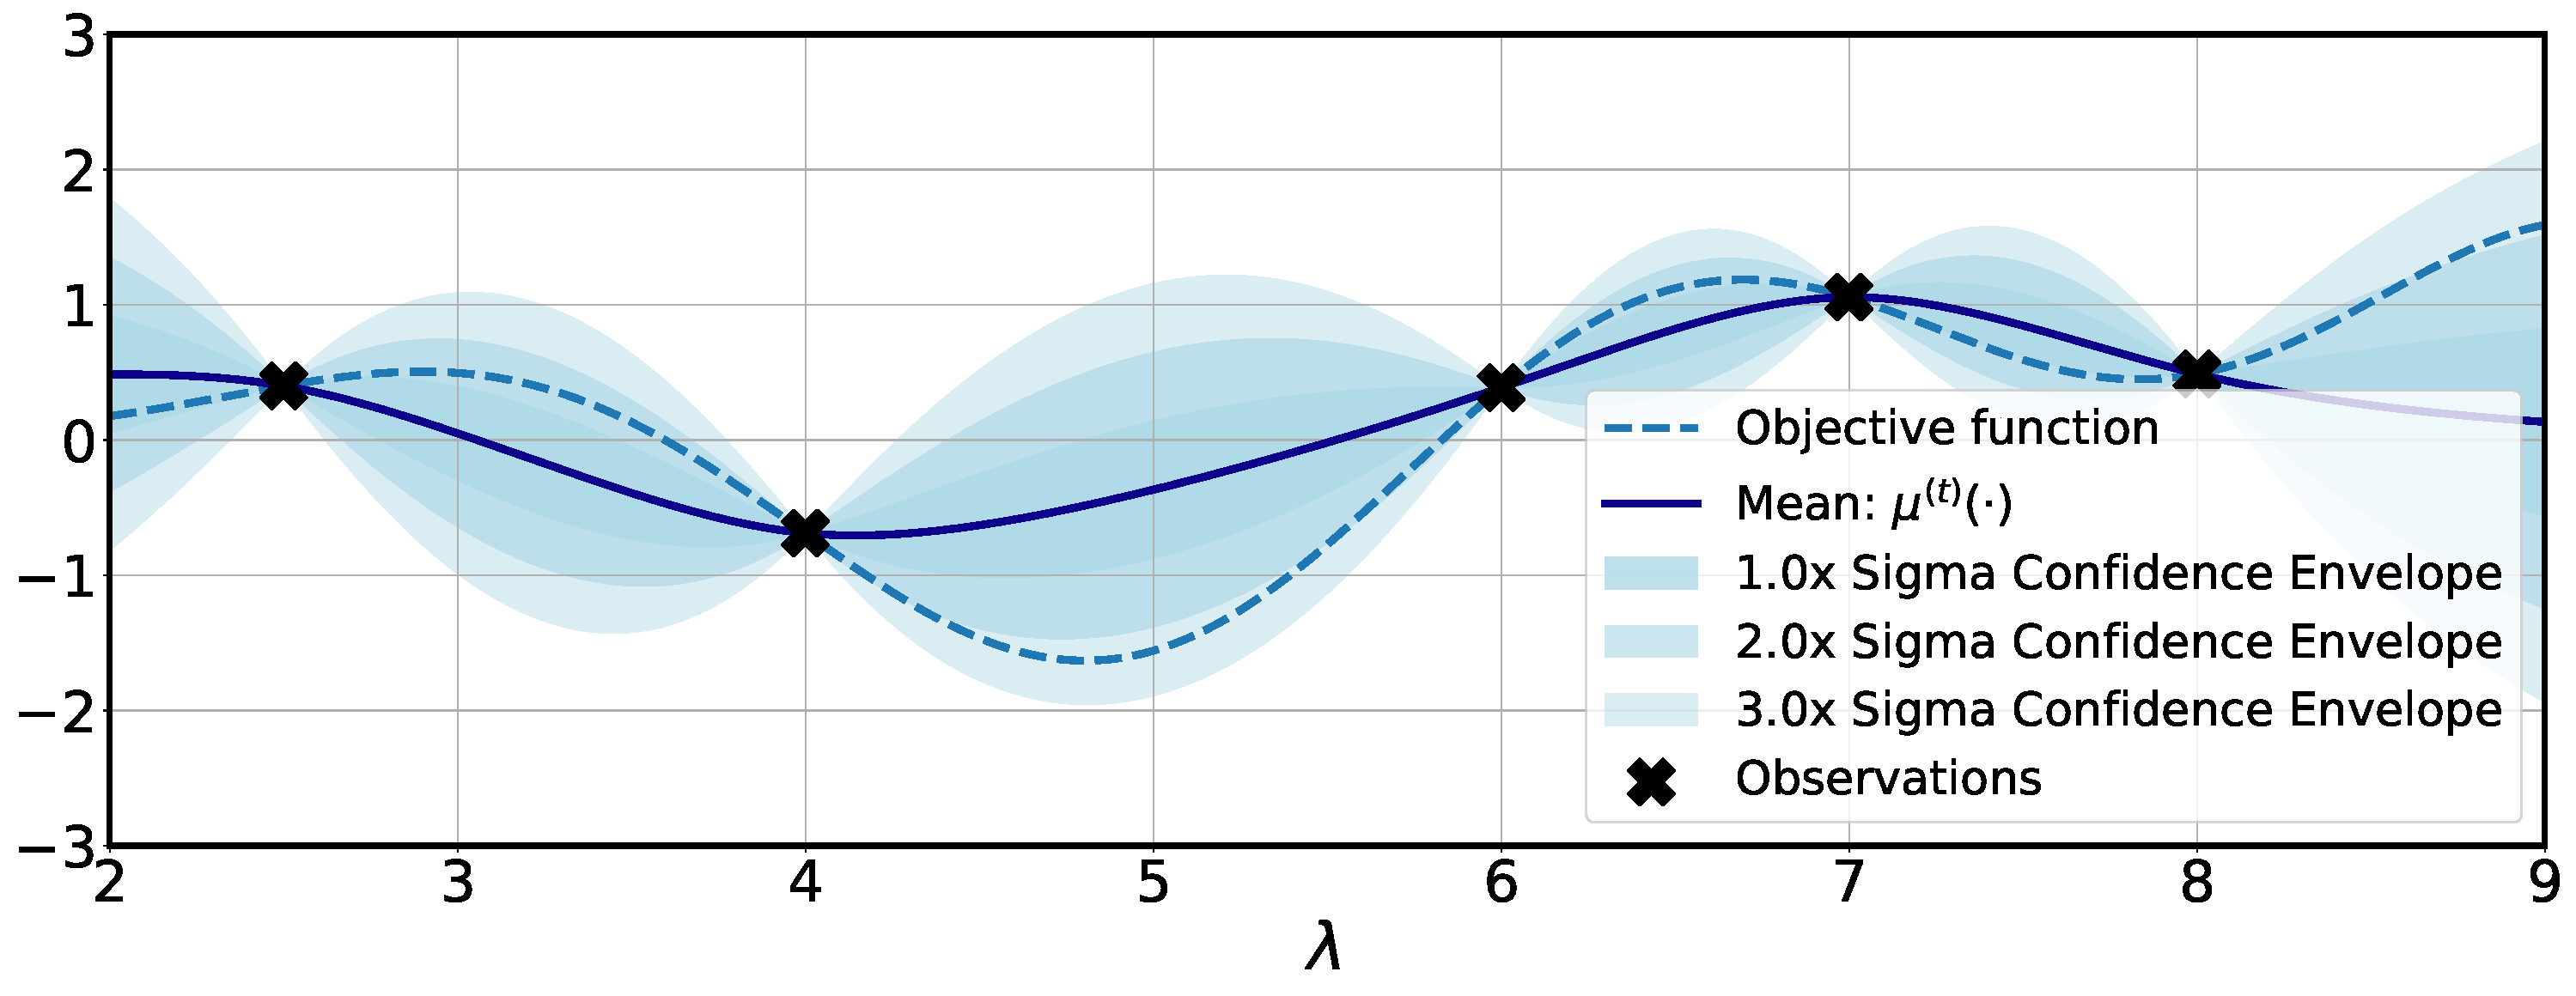
\includegraphics[width=\textwidth, height=0.7\textheight, keepaspectratio=true]{images/acq_func_images/lookahead/look_ahead_1.pdf}}
  \only<2>{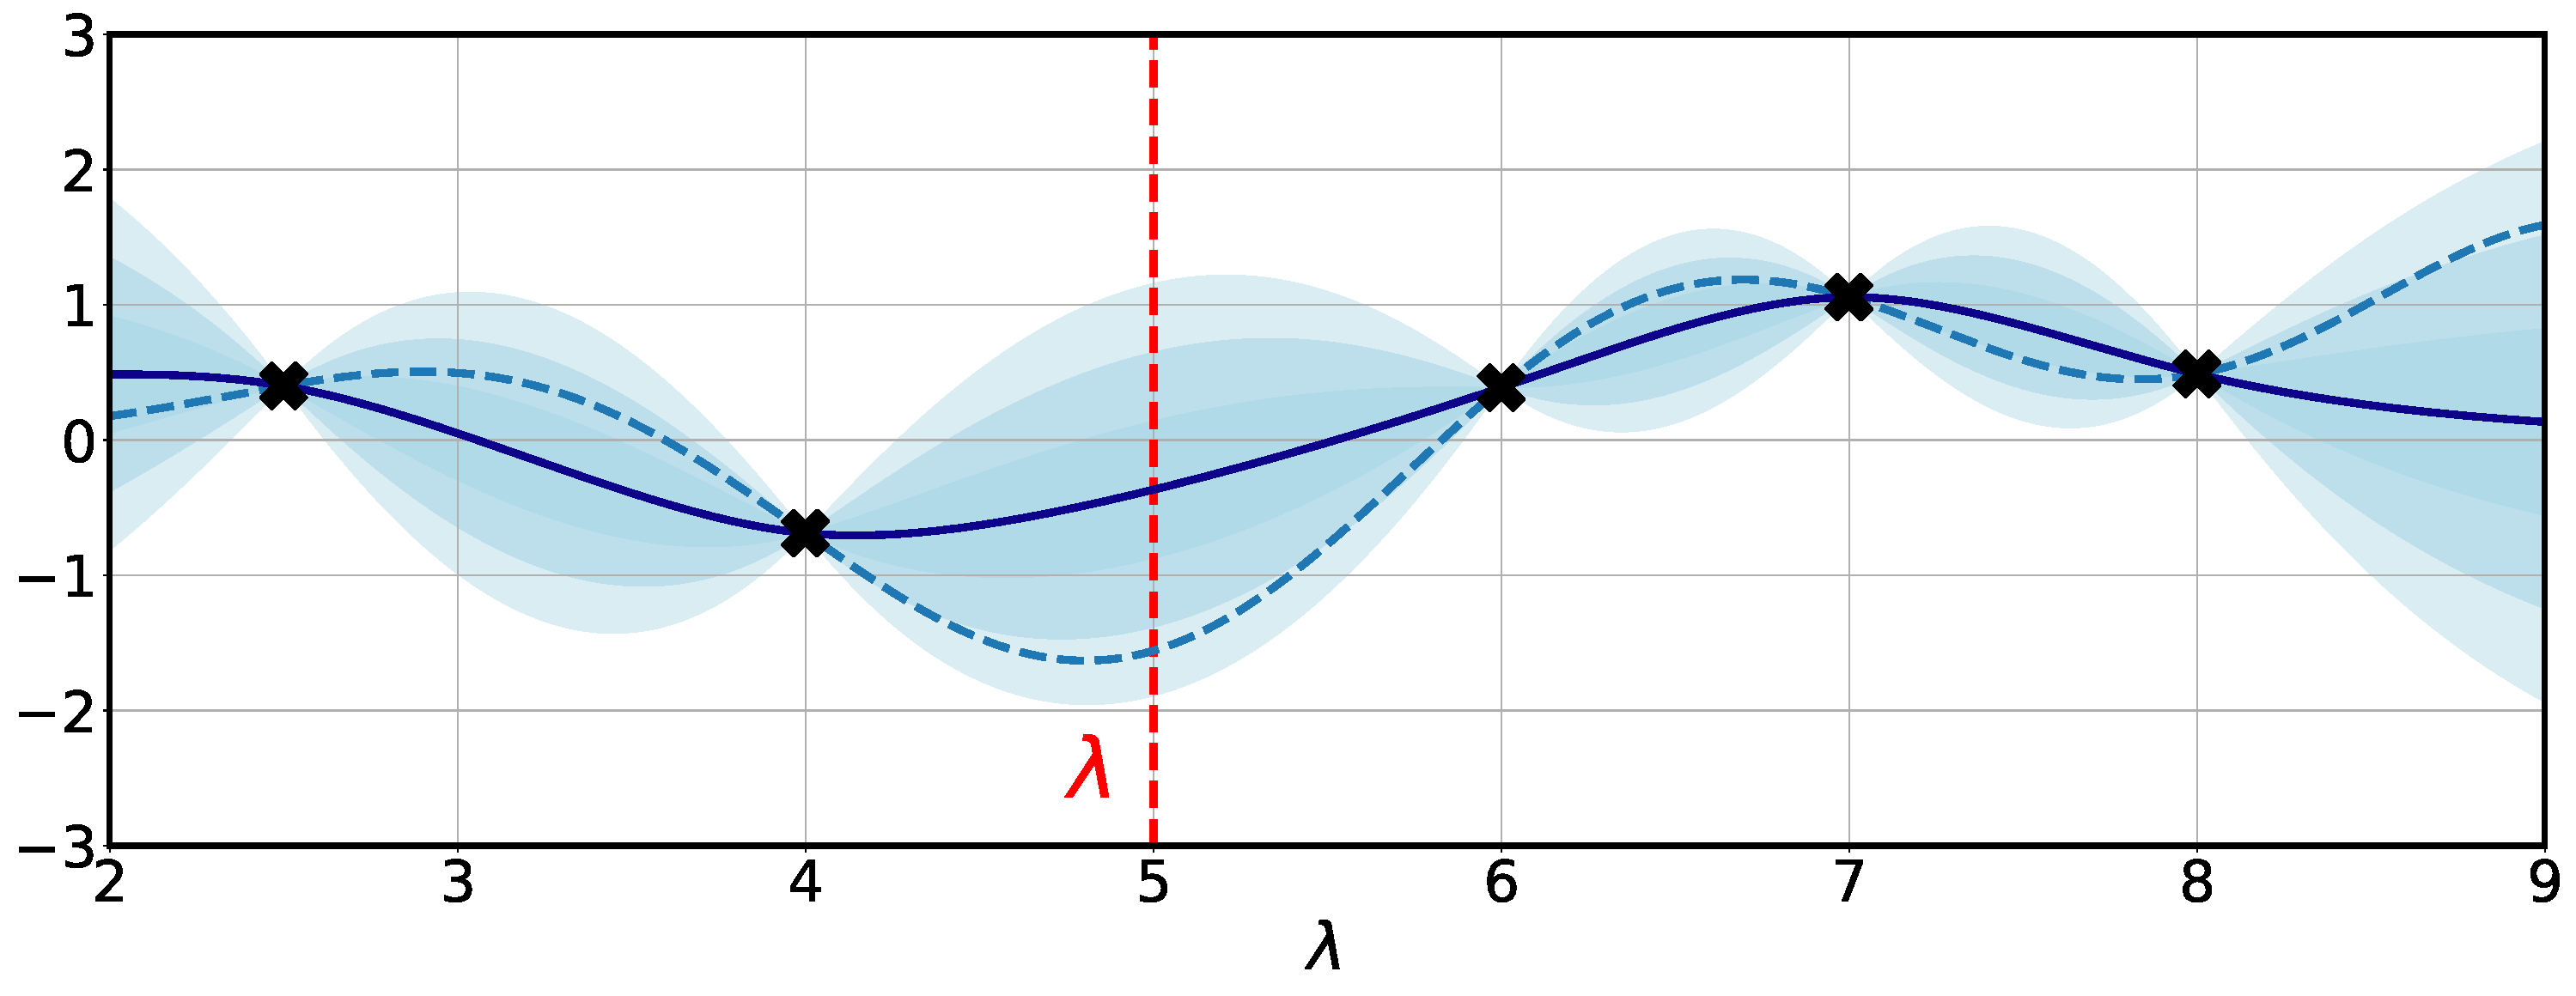
\includegraphics[width=\textwidth, height=0.7\textheight, keepaspectratio=true]{images/acq_func_images/lookahead/look_ahead_2.pdf}}
  \only<3>{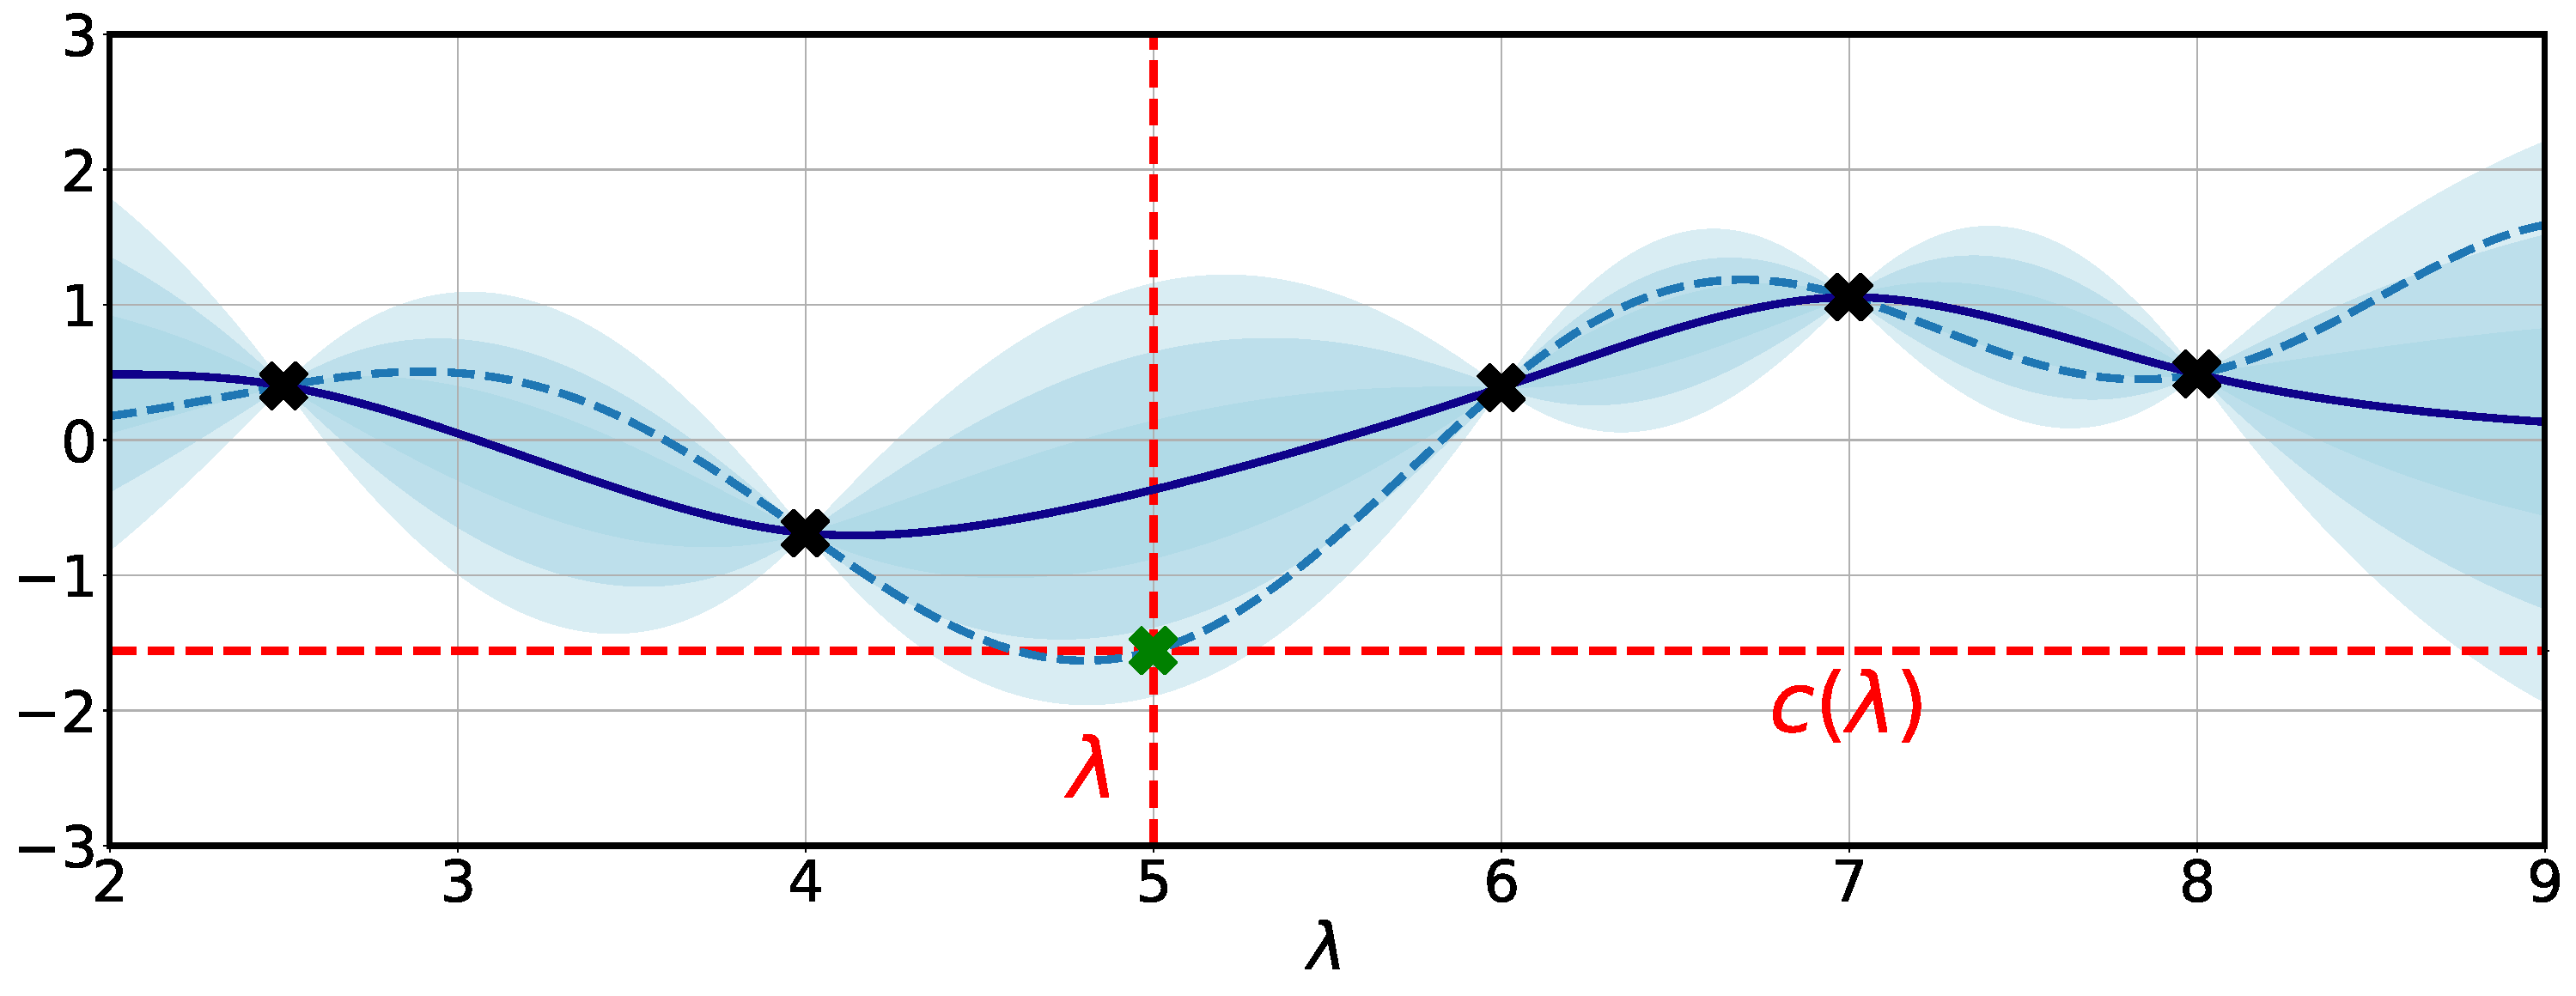
\includegraphics[width=\textwidth, height=0.7\textheight, keepaspectratio=true]{images/acq_func_images/lookahead/look_ahead_3.pdf}}
  \only<4>{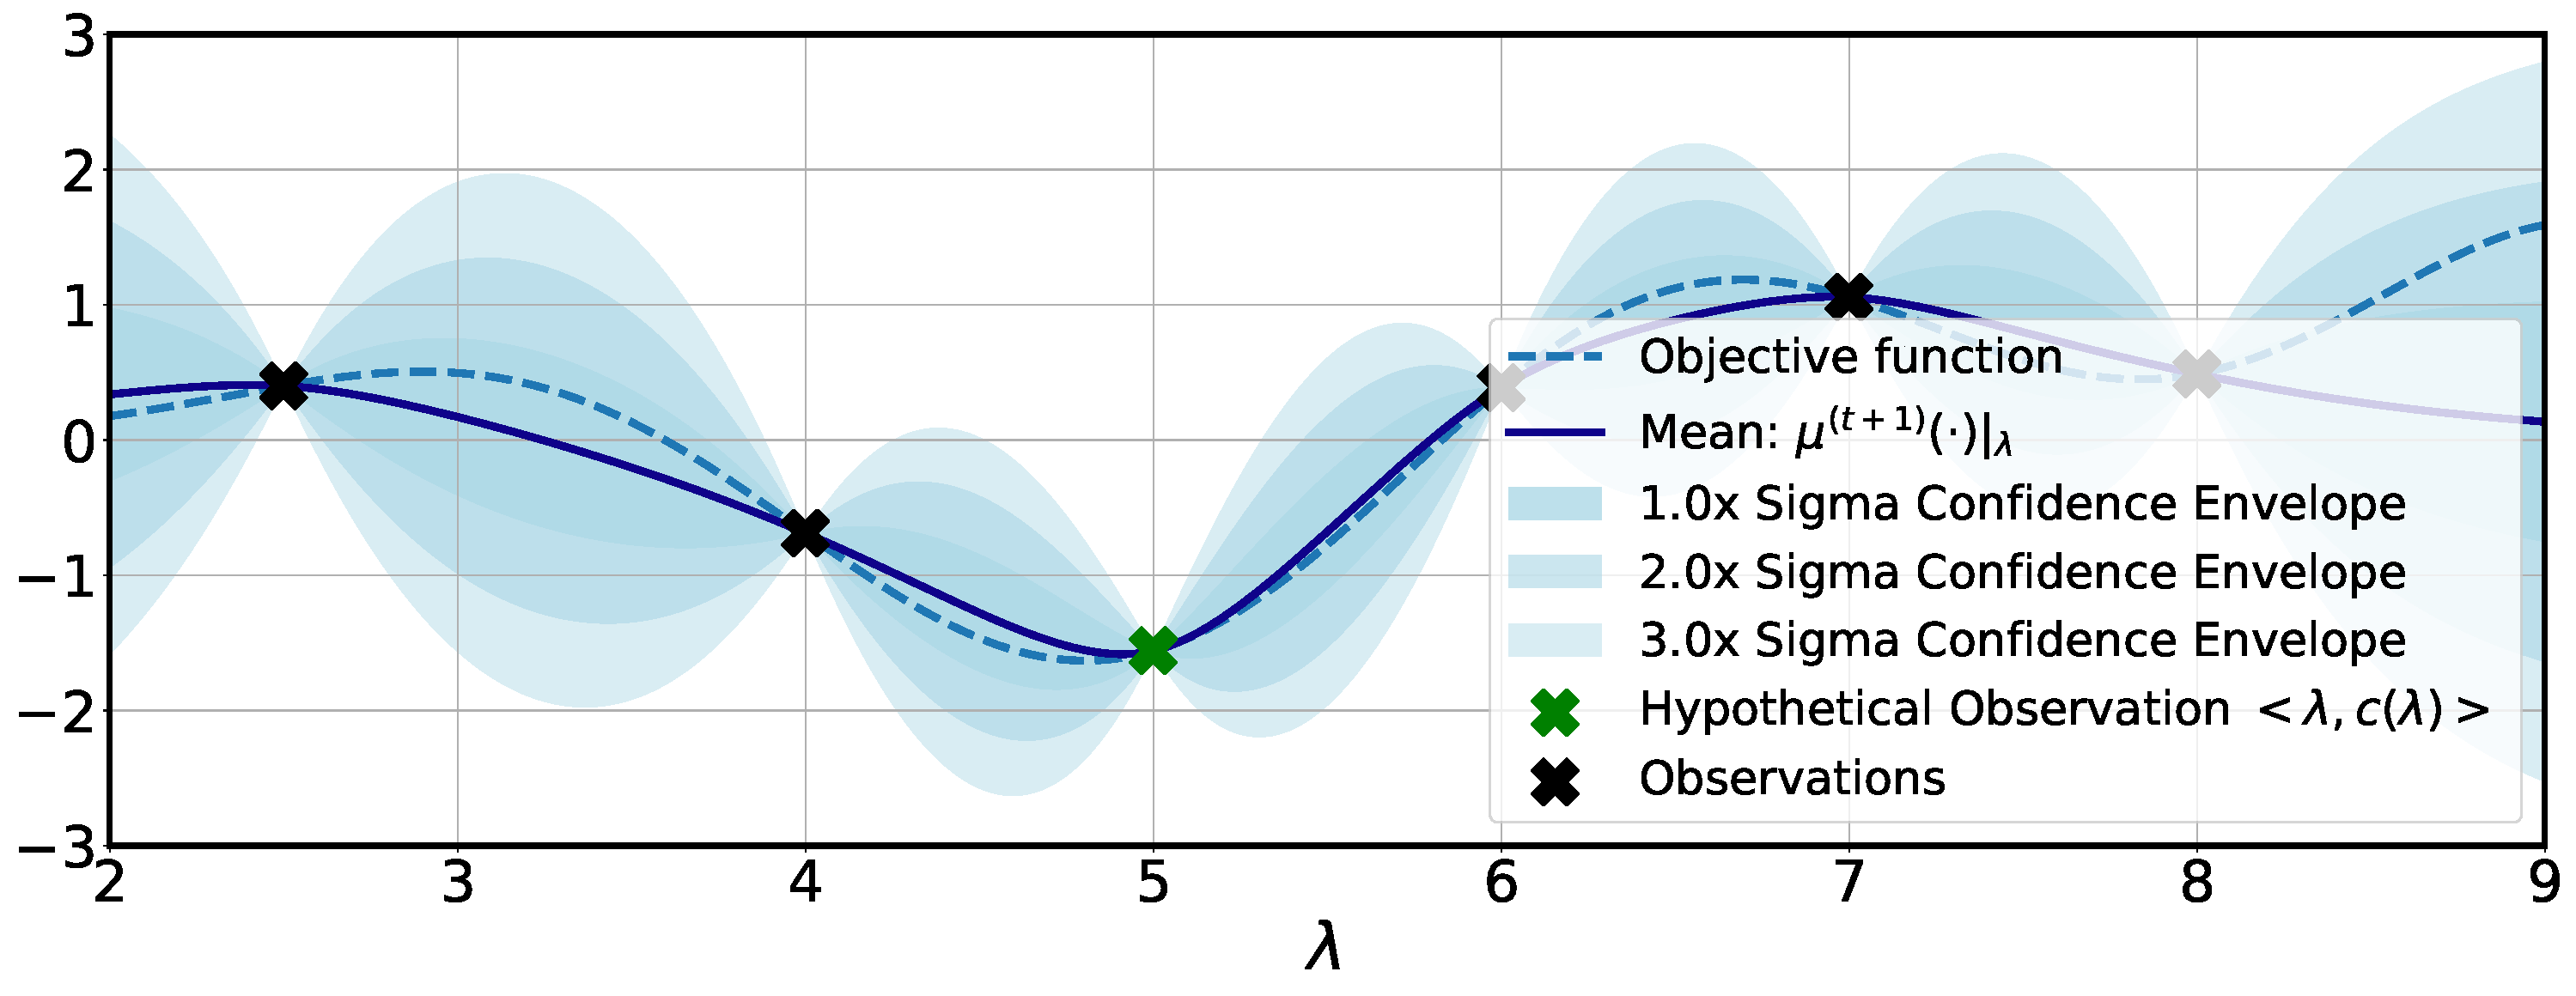
\includegraphics[width=\textwidth, height=0.7\textheight, keepaspectratio=true]{images/acq_func_images/lookahead/look_ahead_4.pdf}}
\end{overlayarea}

\only<1>{Given the surrogate $\iter[\bocount]{\surro}$ fit at iteration $\bocount$}
\only<2>{Imagine that we sample at a random configuration $\conf$}
\only<3>{We would then observe the cost $\cost(\conf)$ at this imaginary configuration $\conf$}
\only<4>{With this hypothetical data point at $\lambda$, we'd have this  \alert{1-step lookahead surrogate $\iter[\bocount+1]{\surro}{\!\given_{\!\conf}}(\cdot)$}}

\end{frame}
%-----------------------------------------------------------------------   
\begin{frame}[c]{Visualization of How Different the Lookahead Surrogate Can Be}

% \begin{figure}
  \centering
  \begin{tikzpicture}

    \node<+> (img5) {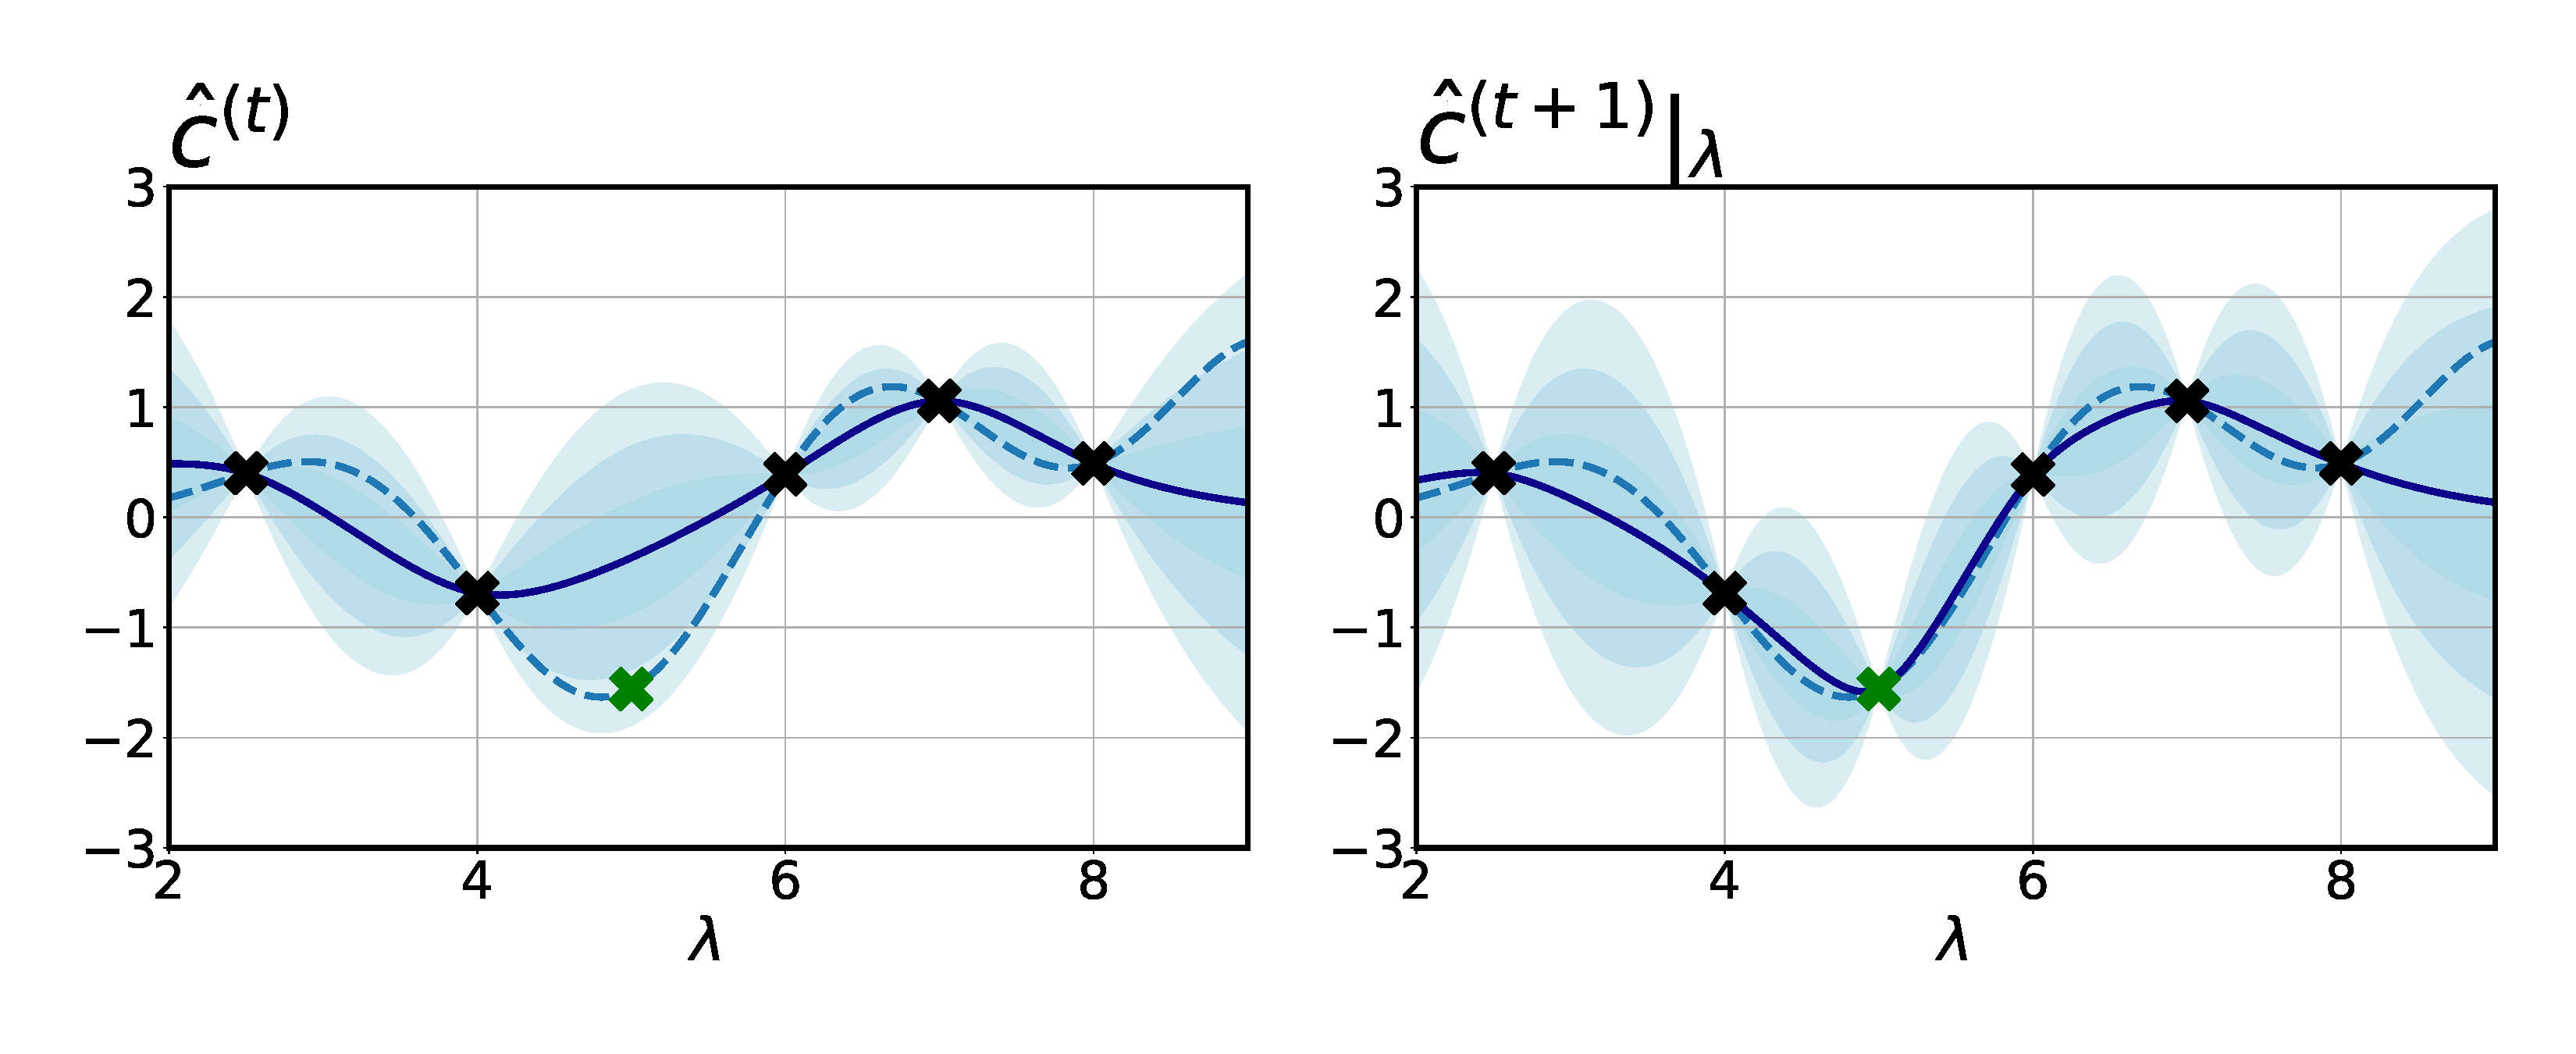
\includegraphics[width=\textwidth, height=0.7\textheight, keepaspectratio=true]{images/acq_func_images/lookahead/look_ahead_5.pdf}};
    \node<.> [below=0.01\belowcaptionskip of img5, align=center]{A comparison of $\iter{\surro}(\cdot)$ and $\iter[\bocount+1]{\surro}{\!\given_{\!\conf}}(\cdot)$ for a given $\conf$.};
    
    \node<+> (img6) {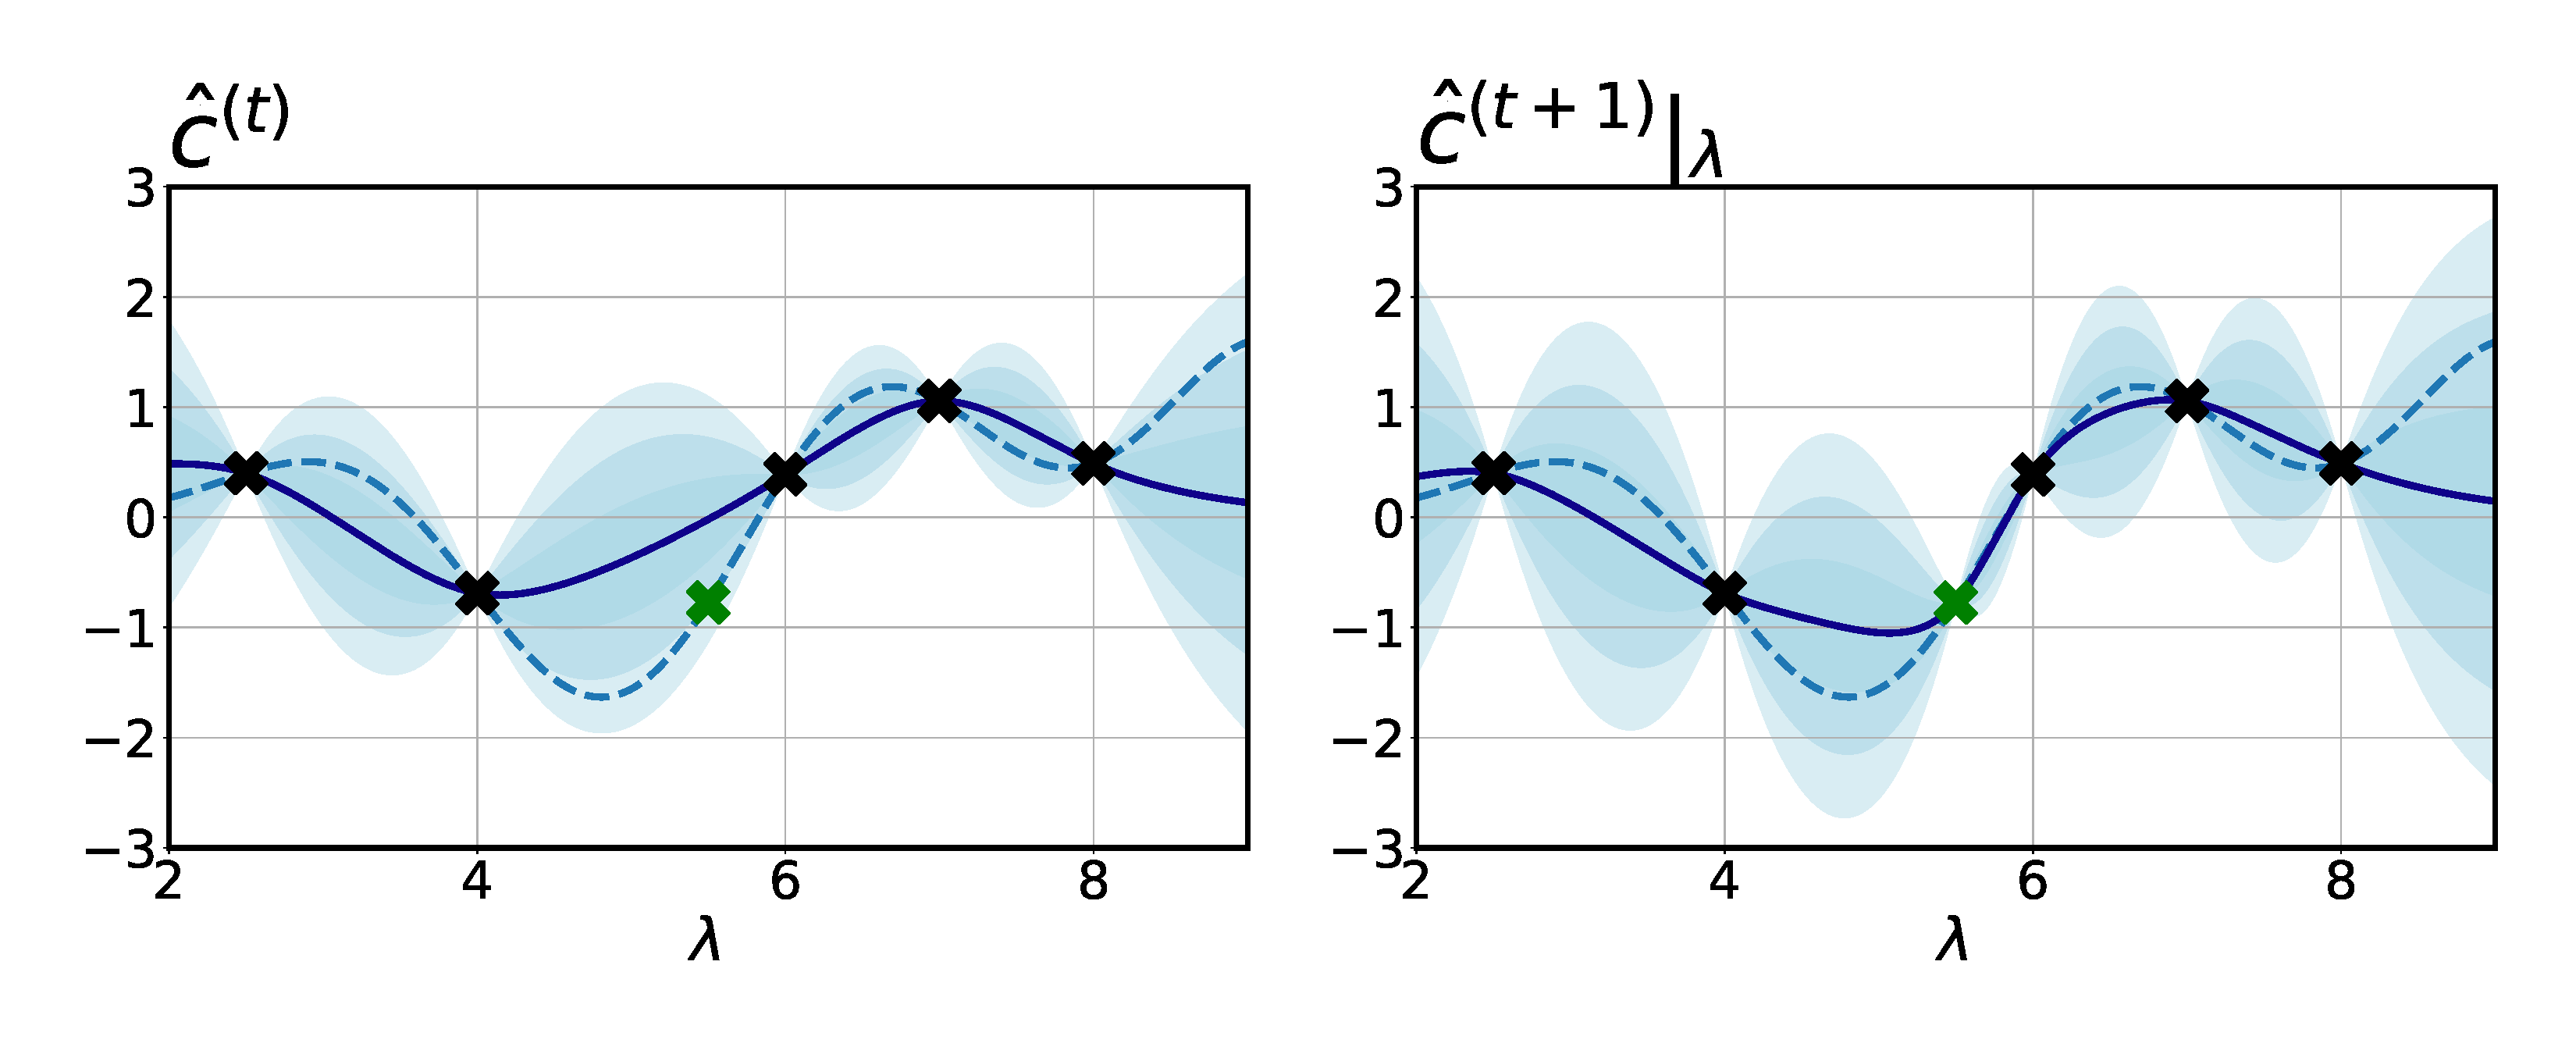
\includegraphics[width=\textwidth, height=0.7\textheight, keepaspectratio=true]{images/acq_func_images/lookahead/look_ahead_6.pdf}};
    \node<.> [below=0.01\belowcaptionskip of img6, align=center]{A comparison of $\iter{\surro}(\cdot)$ and $\iter[\bocount+1]{\surro}{\!\given_{\!\conf}}(\cdot)$ for a given $\conf$.};
    
    \node<+> (img7) {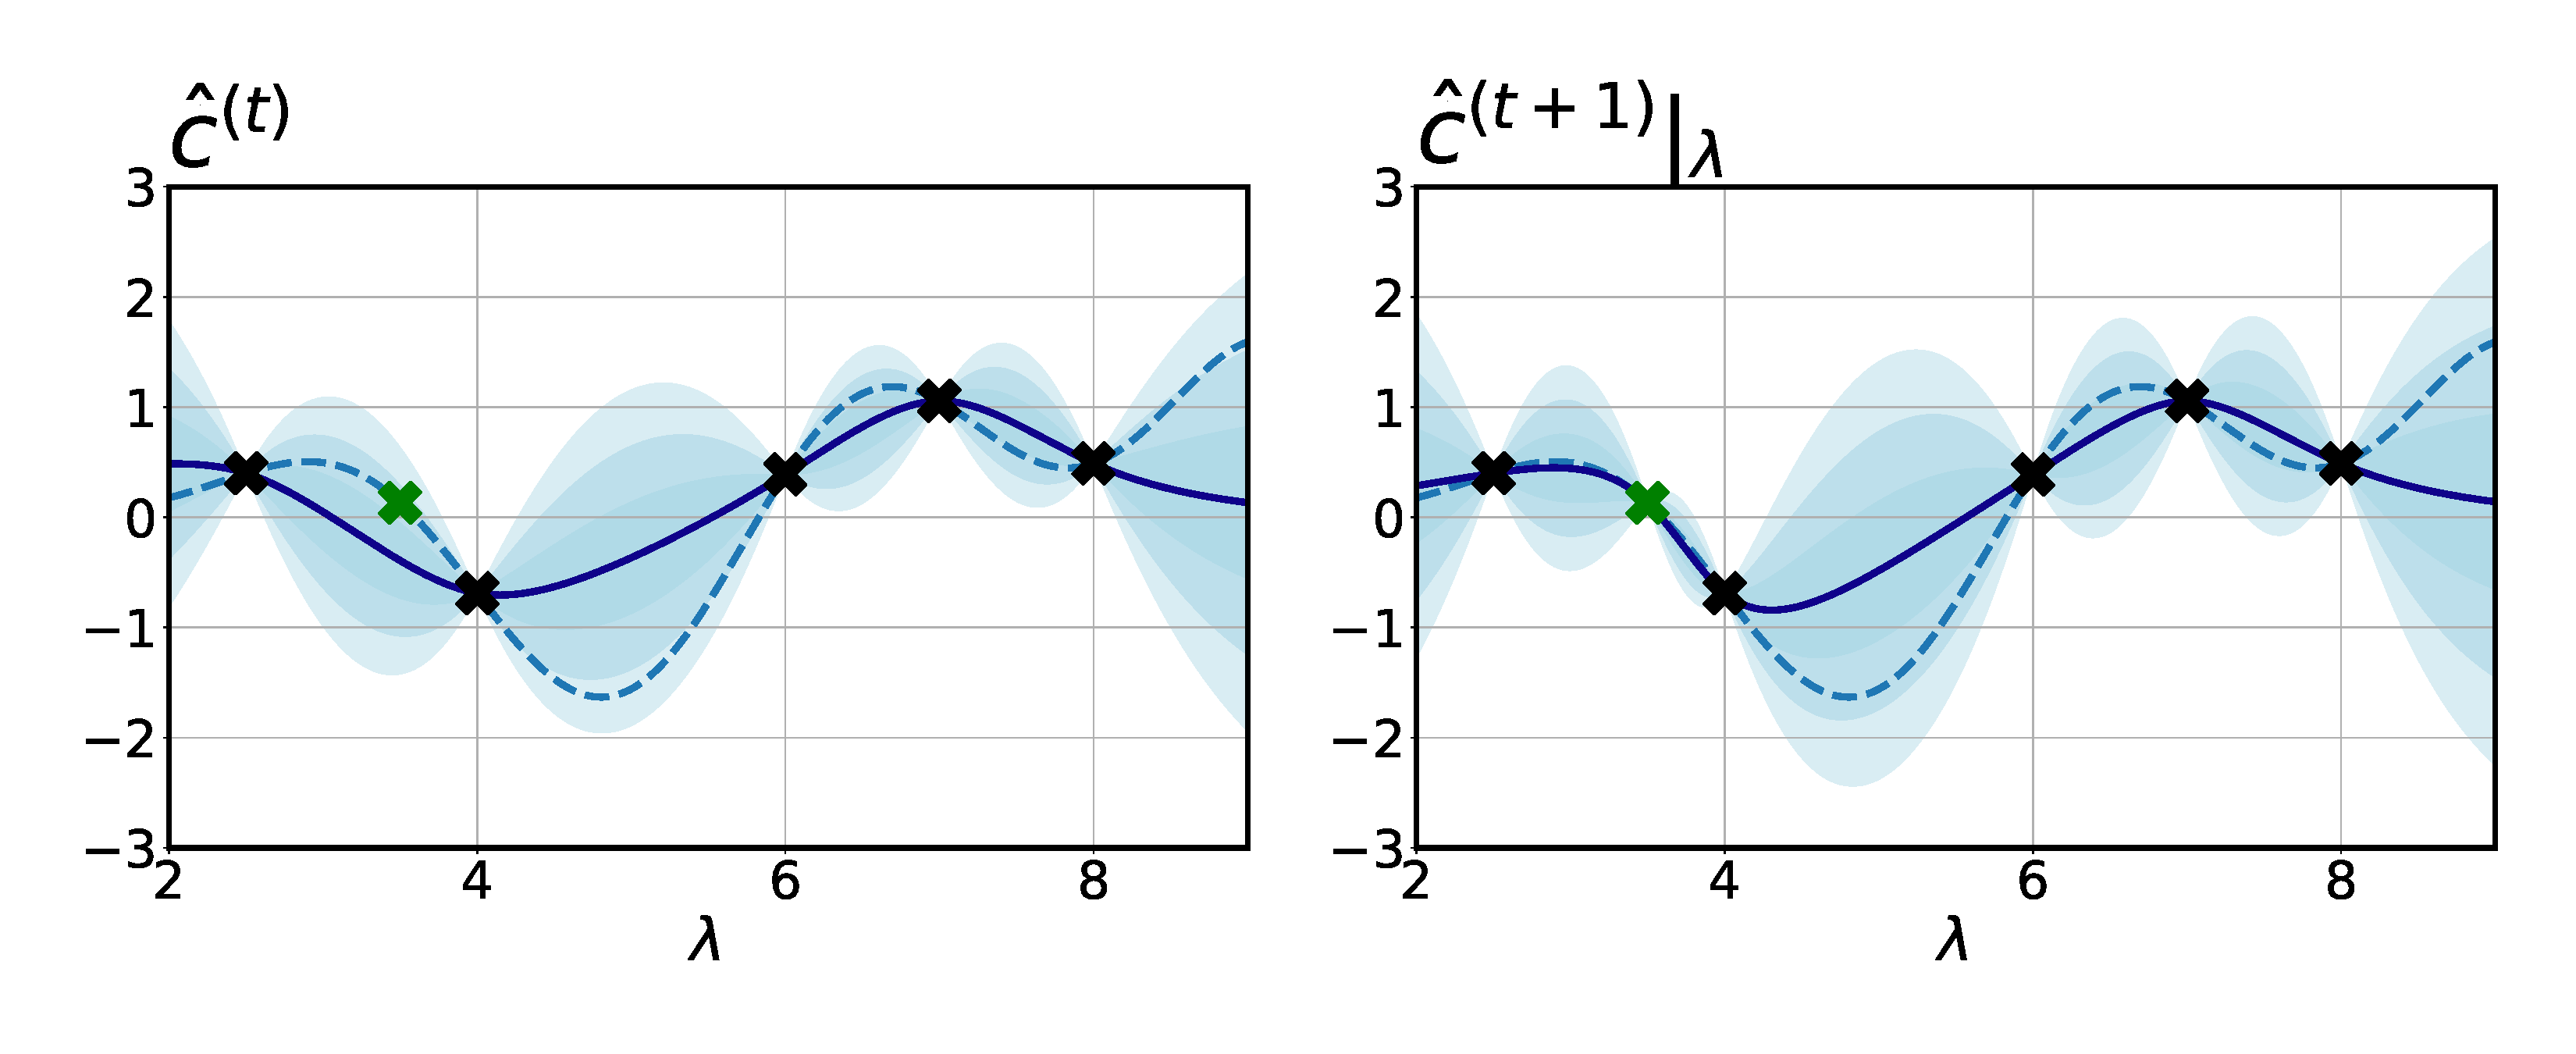
\includegraphics[width=\textwidth, height=0.7\textheight, keepaspectratio=true]{images/acq_func_images/lookahead/look_ahead_7.pdf}};
    \node<.> [below=0.01\belowcaptionskip of img7, align=center]{A comparison of $\iter{\surro}(\cdot)$ and $\iter[\bocount+1]{\surro}{\!\given_{\!\conf}}(\cdot)$ for a given $\conf$.};

\comment{Pardon the inconsistent label for the vertical red line - it's a bug that would need some time to trace and solve, but should not affect the readability of the plots.}

\comment{Here we are fantasizing how the GP would look like if we had done an actual evaluation at the chosen configuration, i.e. had observed the actual cost incurred for using that configuration.}

\comment{Mean - $\iter[\bocount+1]{\mean} \given_{\conf}$, Variance - $\iter[\bocount+1]{\left(\variance\right)} \given_{\conf}$, Minimum of the mean function - $\iter[\bocount+1]{\left(\mean^*\right)} \given_{\conf}$. It should be noted that all these quantities are now conditionally dependent on our choice of $\conf$, as demonstrated by the | sign next to all these quantities.}

\comment{This distribution is purely hypothetical - as shown by the conditional - and is called a one-step look-ahead. Just a re-statement of the GP's conditional nature at $\bocount+1$. Since we don't actually have the underlying objective function available in real-life scenarios, it is impossible to generate the true look-ahead without actually performing an evaluation.}
  \end{tikzpicture}
% \end{figure}
\end{frame}

%-----------------------------------------------------------------------


\begin{frame}[c]{Knowledge Gradient (KG): Concept}

% \begin{figure}
\centering
\begin{overlayarea}{\textwidth}{0.8\textheight}
  \only<1>{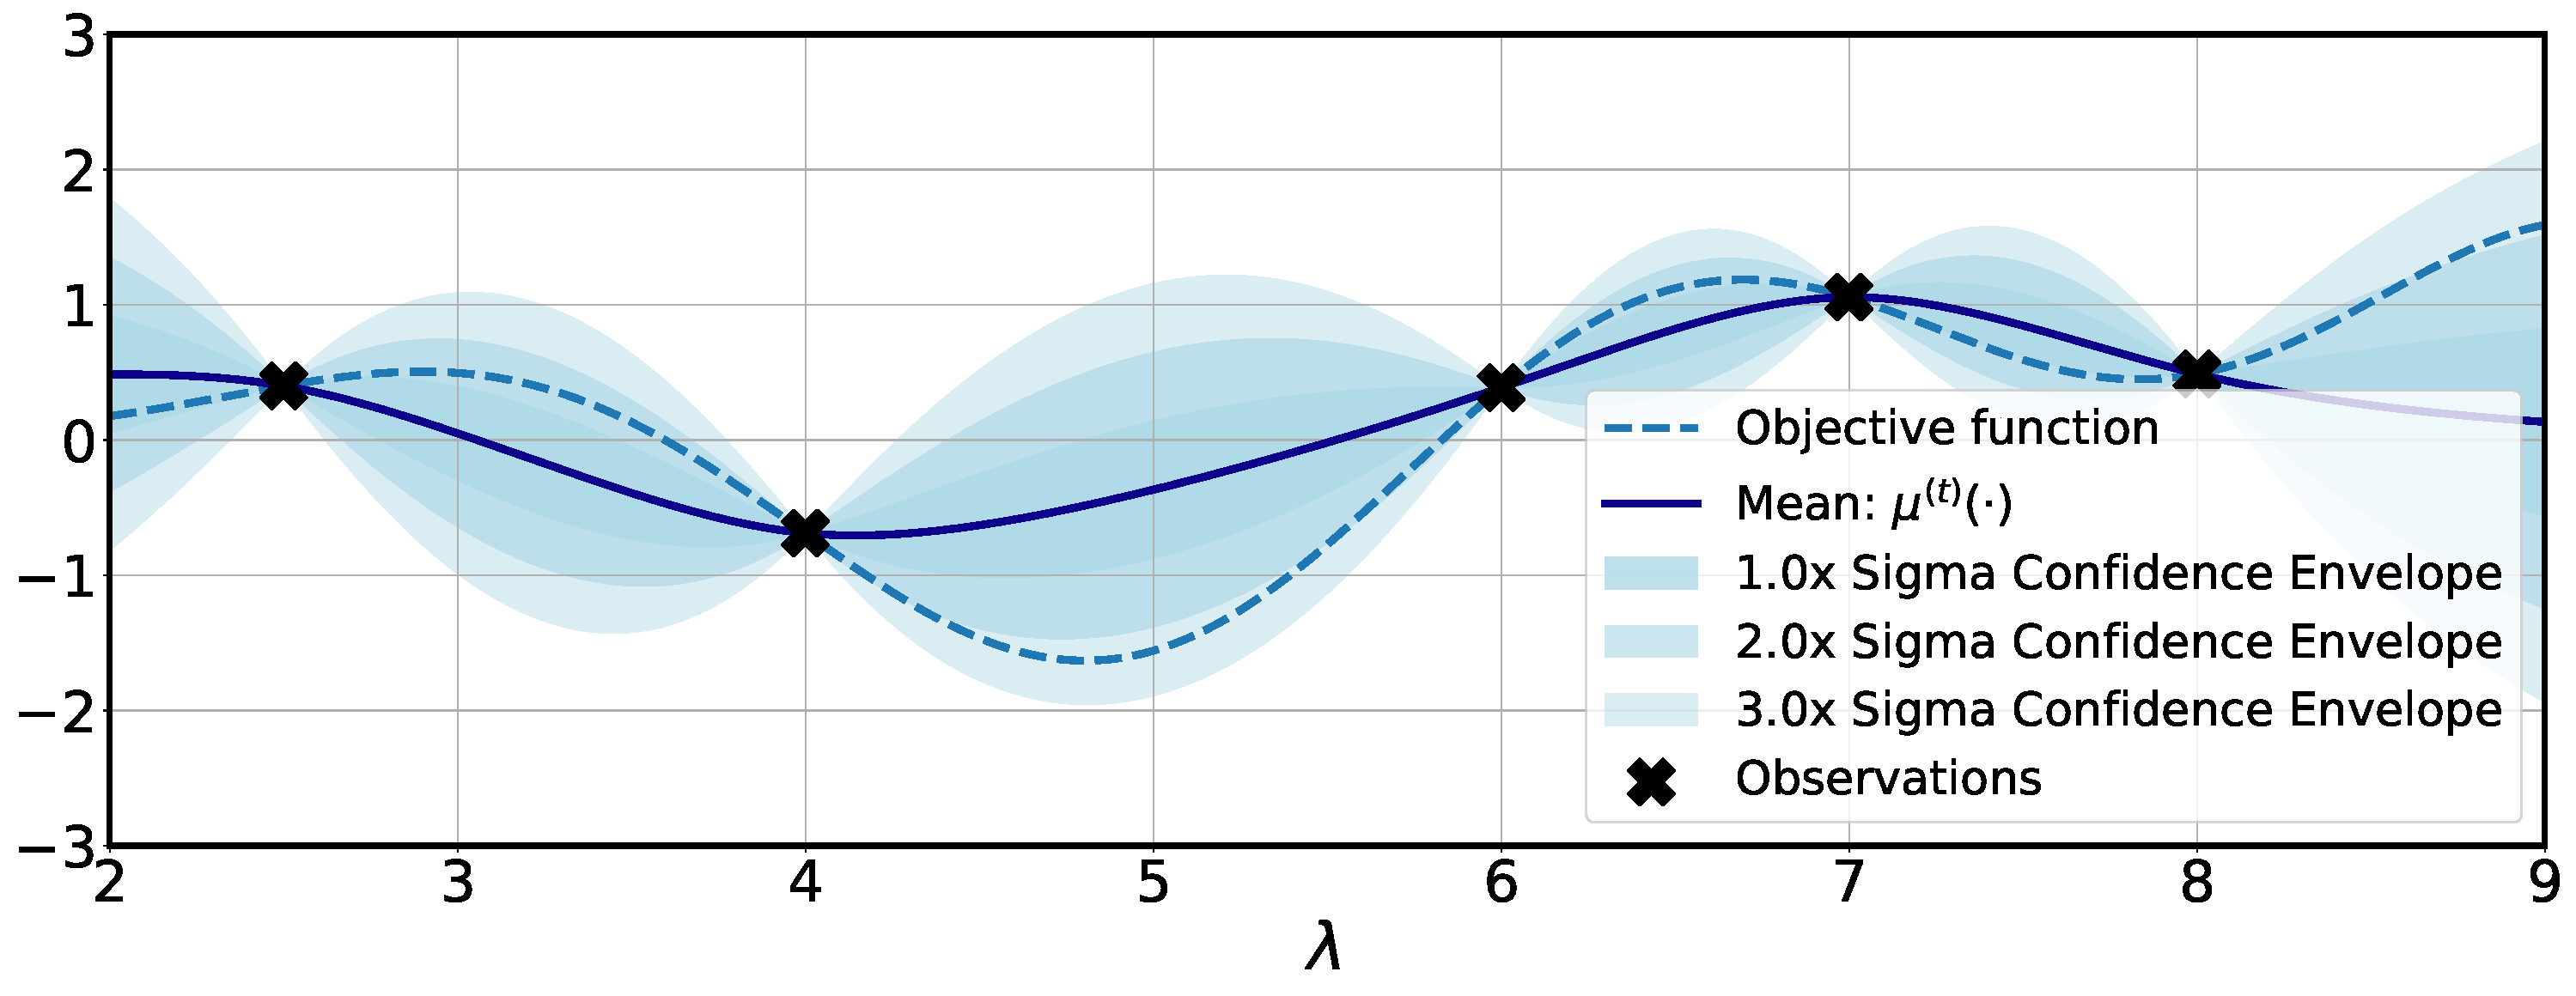
\includegraphics[width=\textwidth, height=0.7\textheight, keepaspectratio=true]{images/acq_func_images/kg/kg_1.pdf}}
  \only<2>{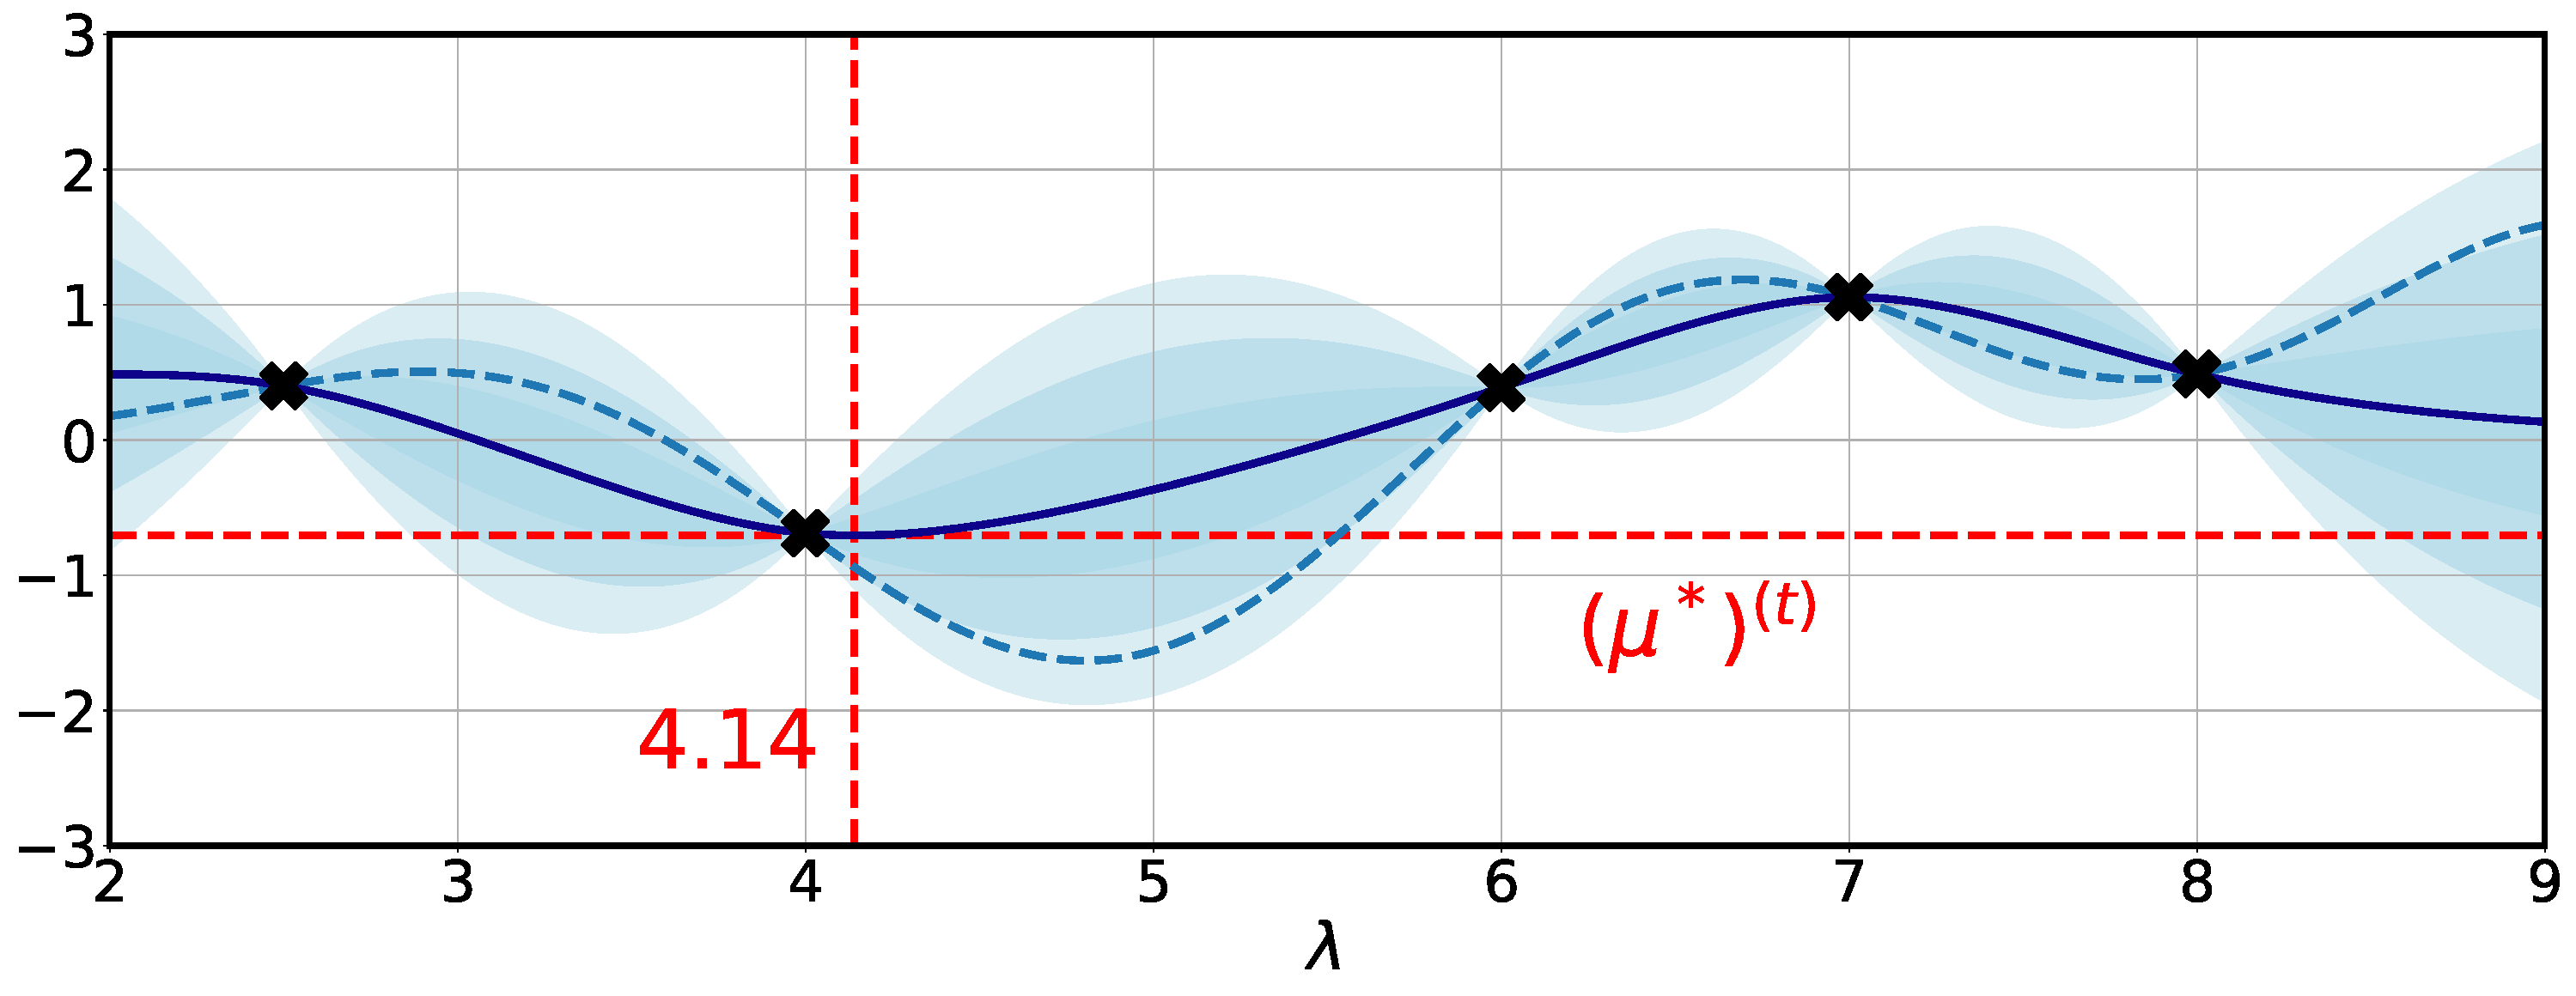
\includegraphics[width=\textwidth, height=0.7\textheight, keepaspectratio=true]{images/acq_func_images/kg/kg_2.pdf}}
  \only<3>{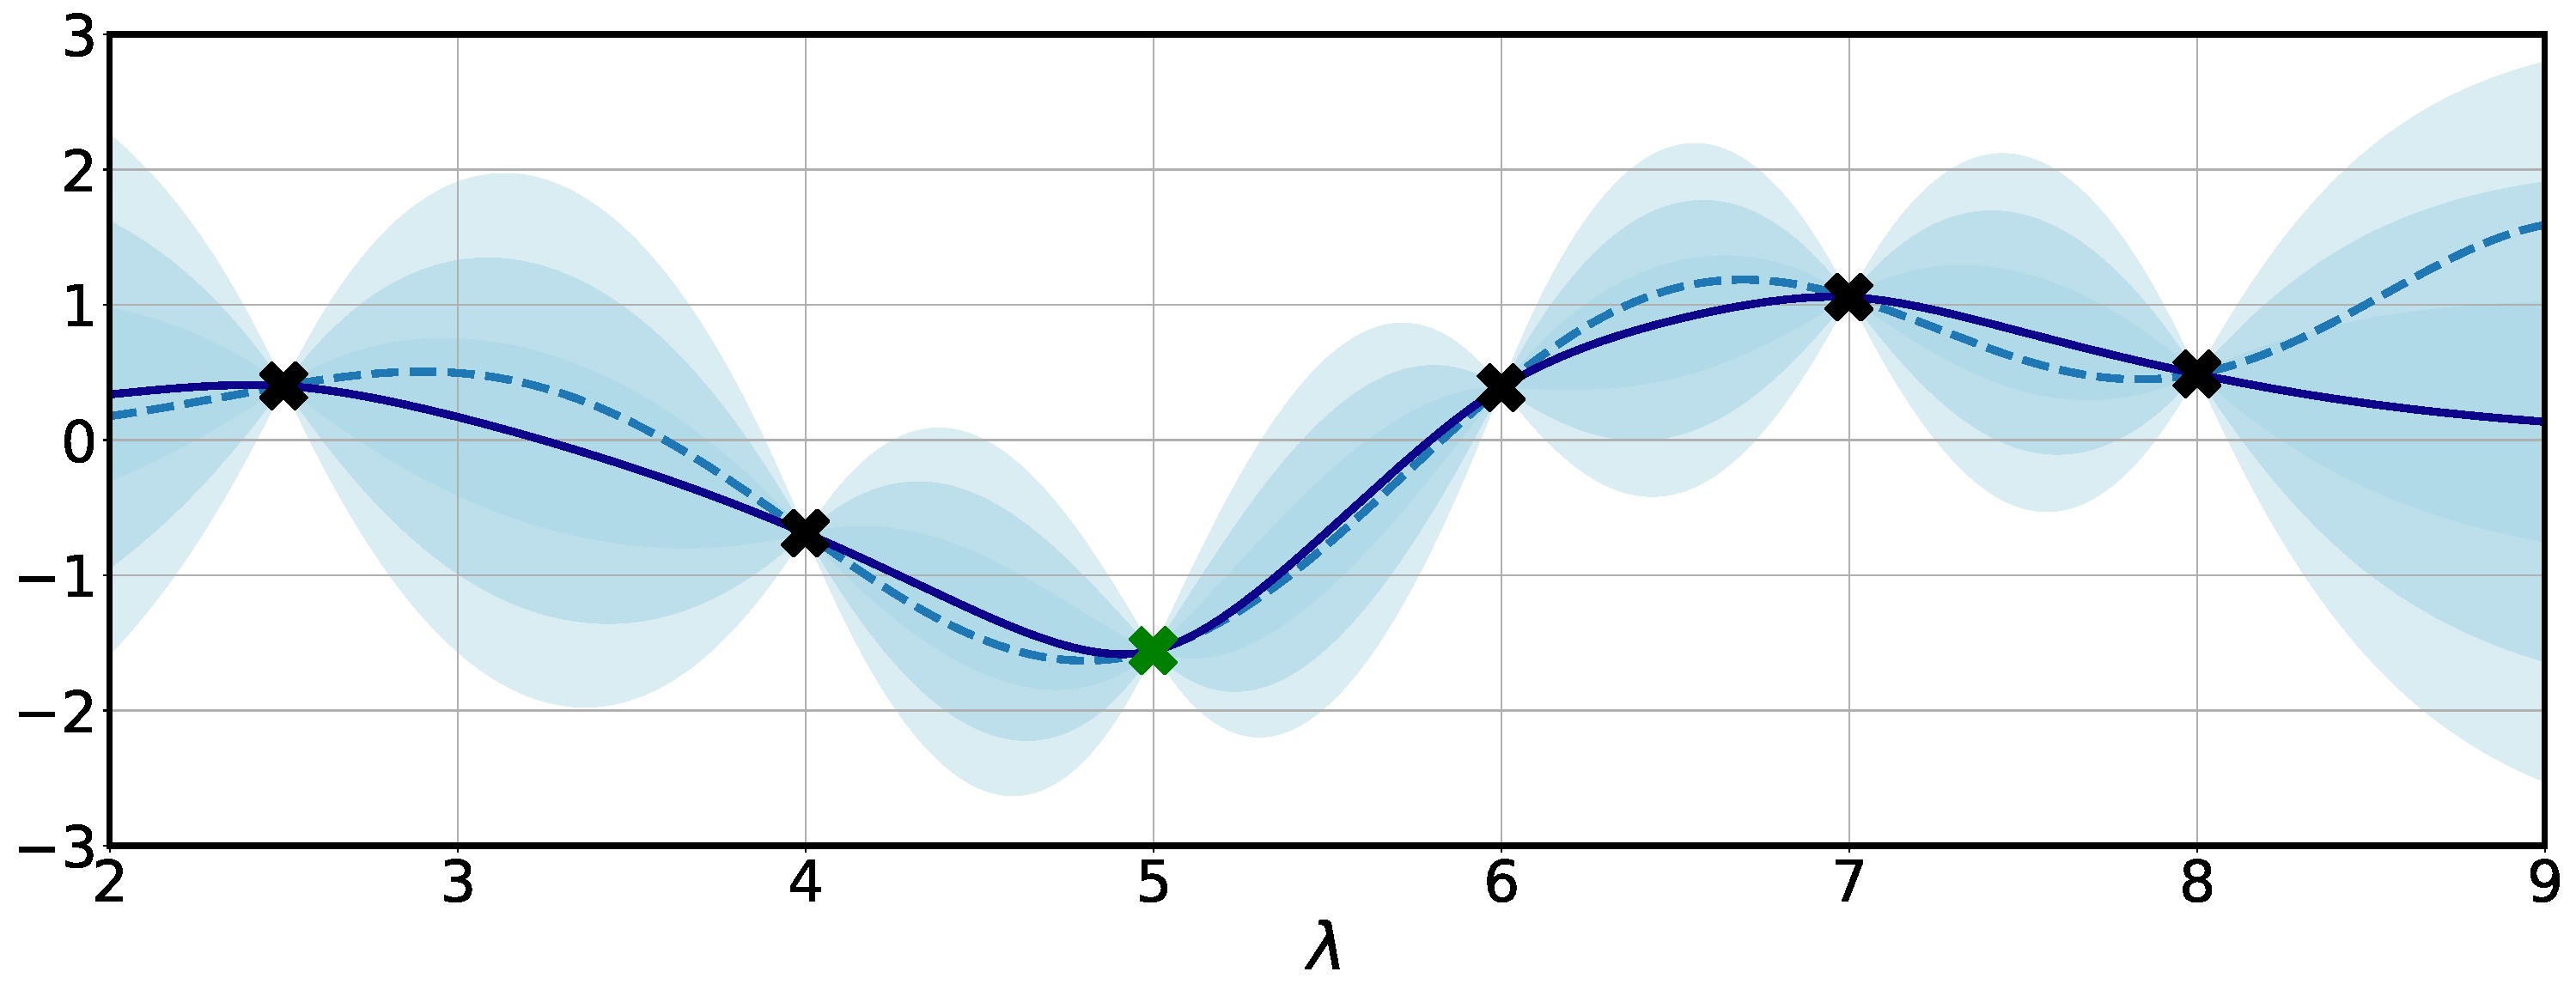
\includegraphics[width=\textwidth, height=0.7\textheight, keepaspectratio=true]{images/acq_func_images/kg/kg_3.pdf}}
  \only<4>{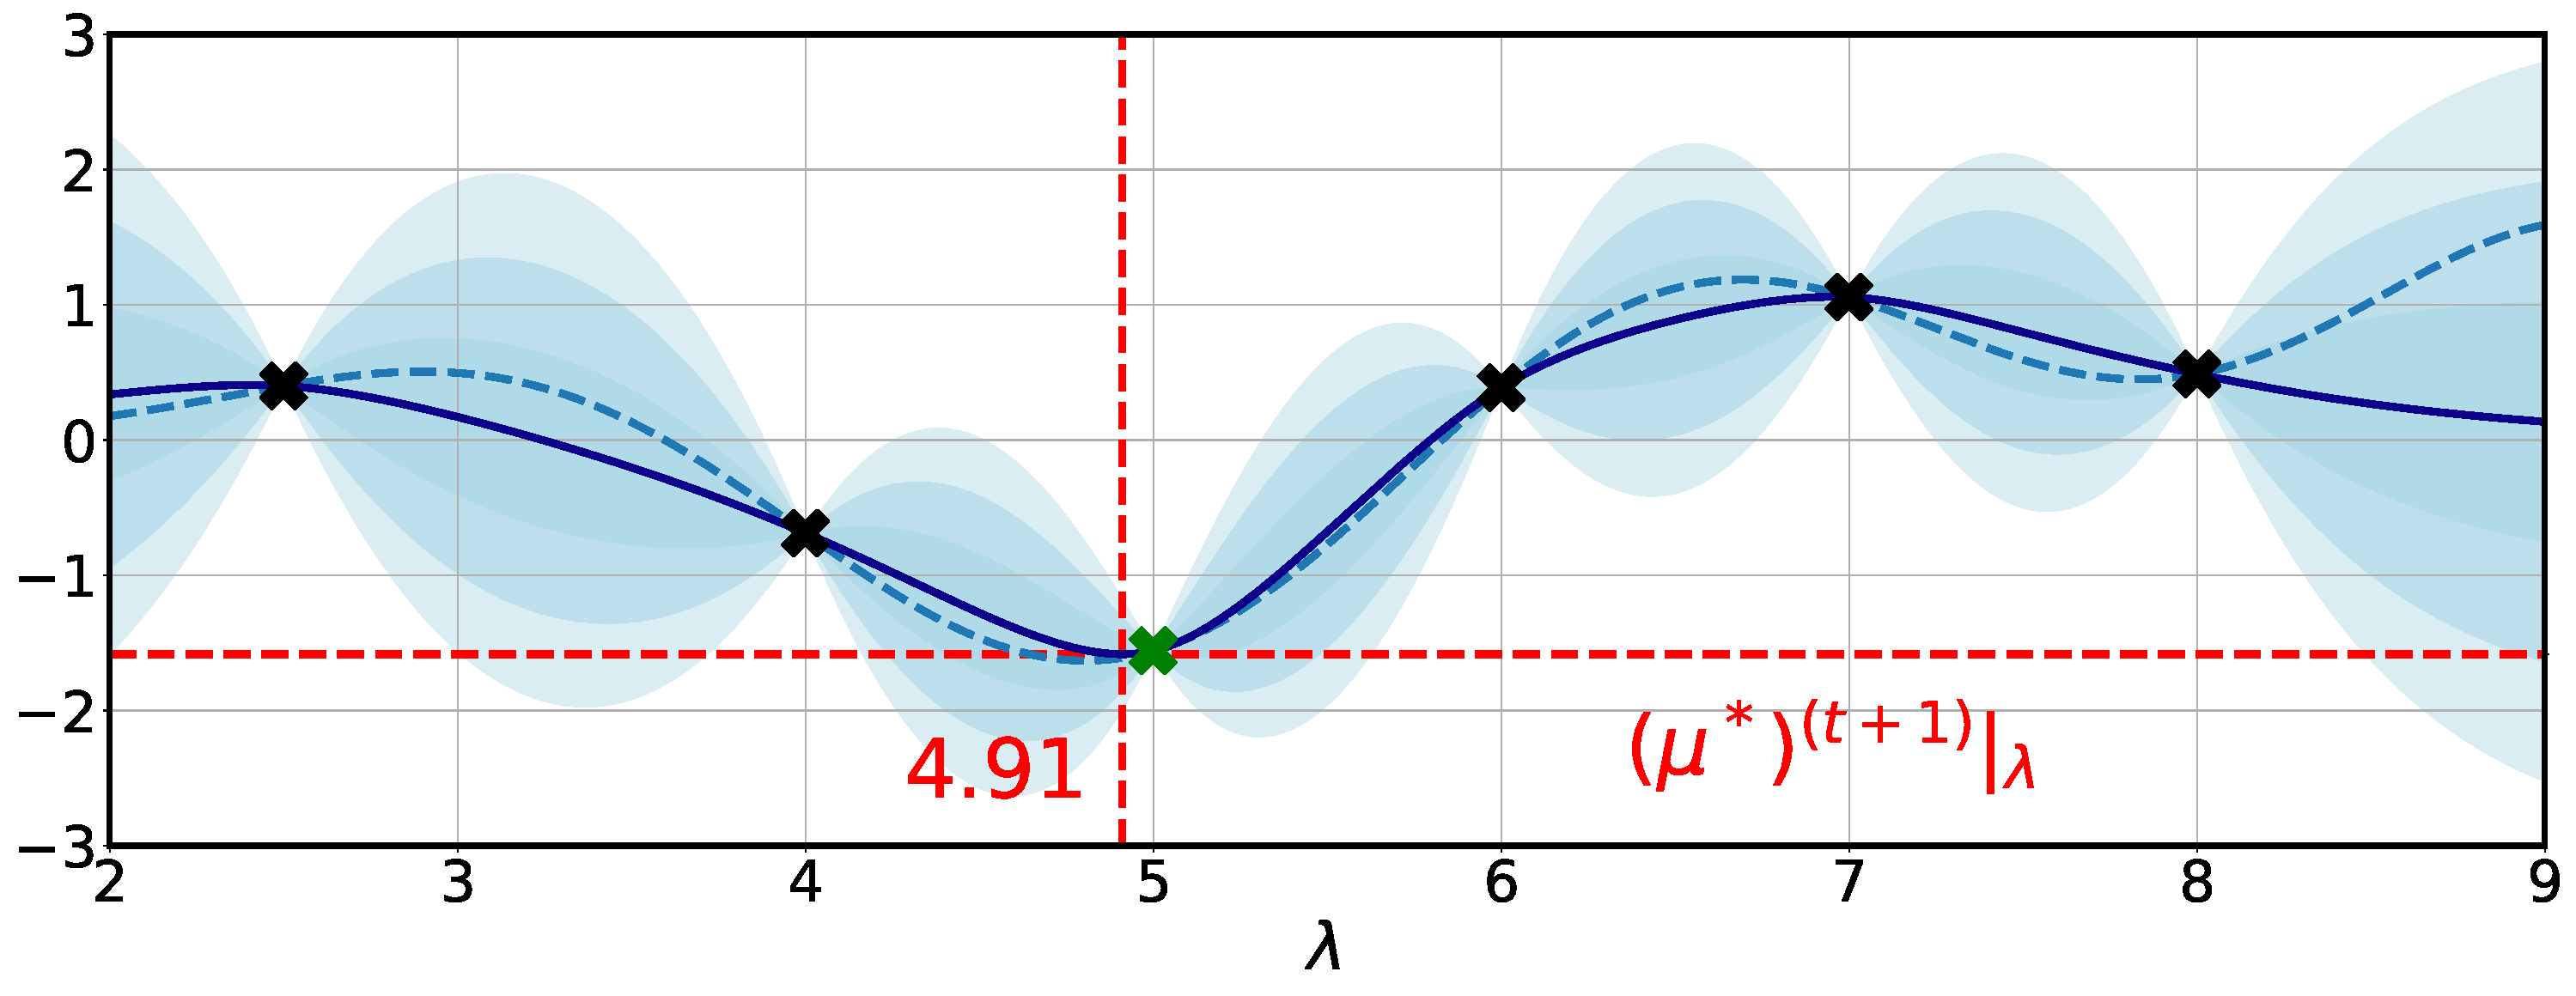
\includegraphics[width=\textwidth, height=0.7\textheight, keepaspectratio=true]{images/acq_func_images/kg/kg_4.pdf}}
  \only<5>{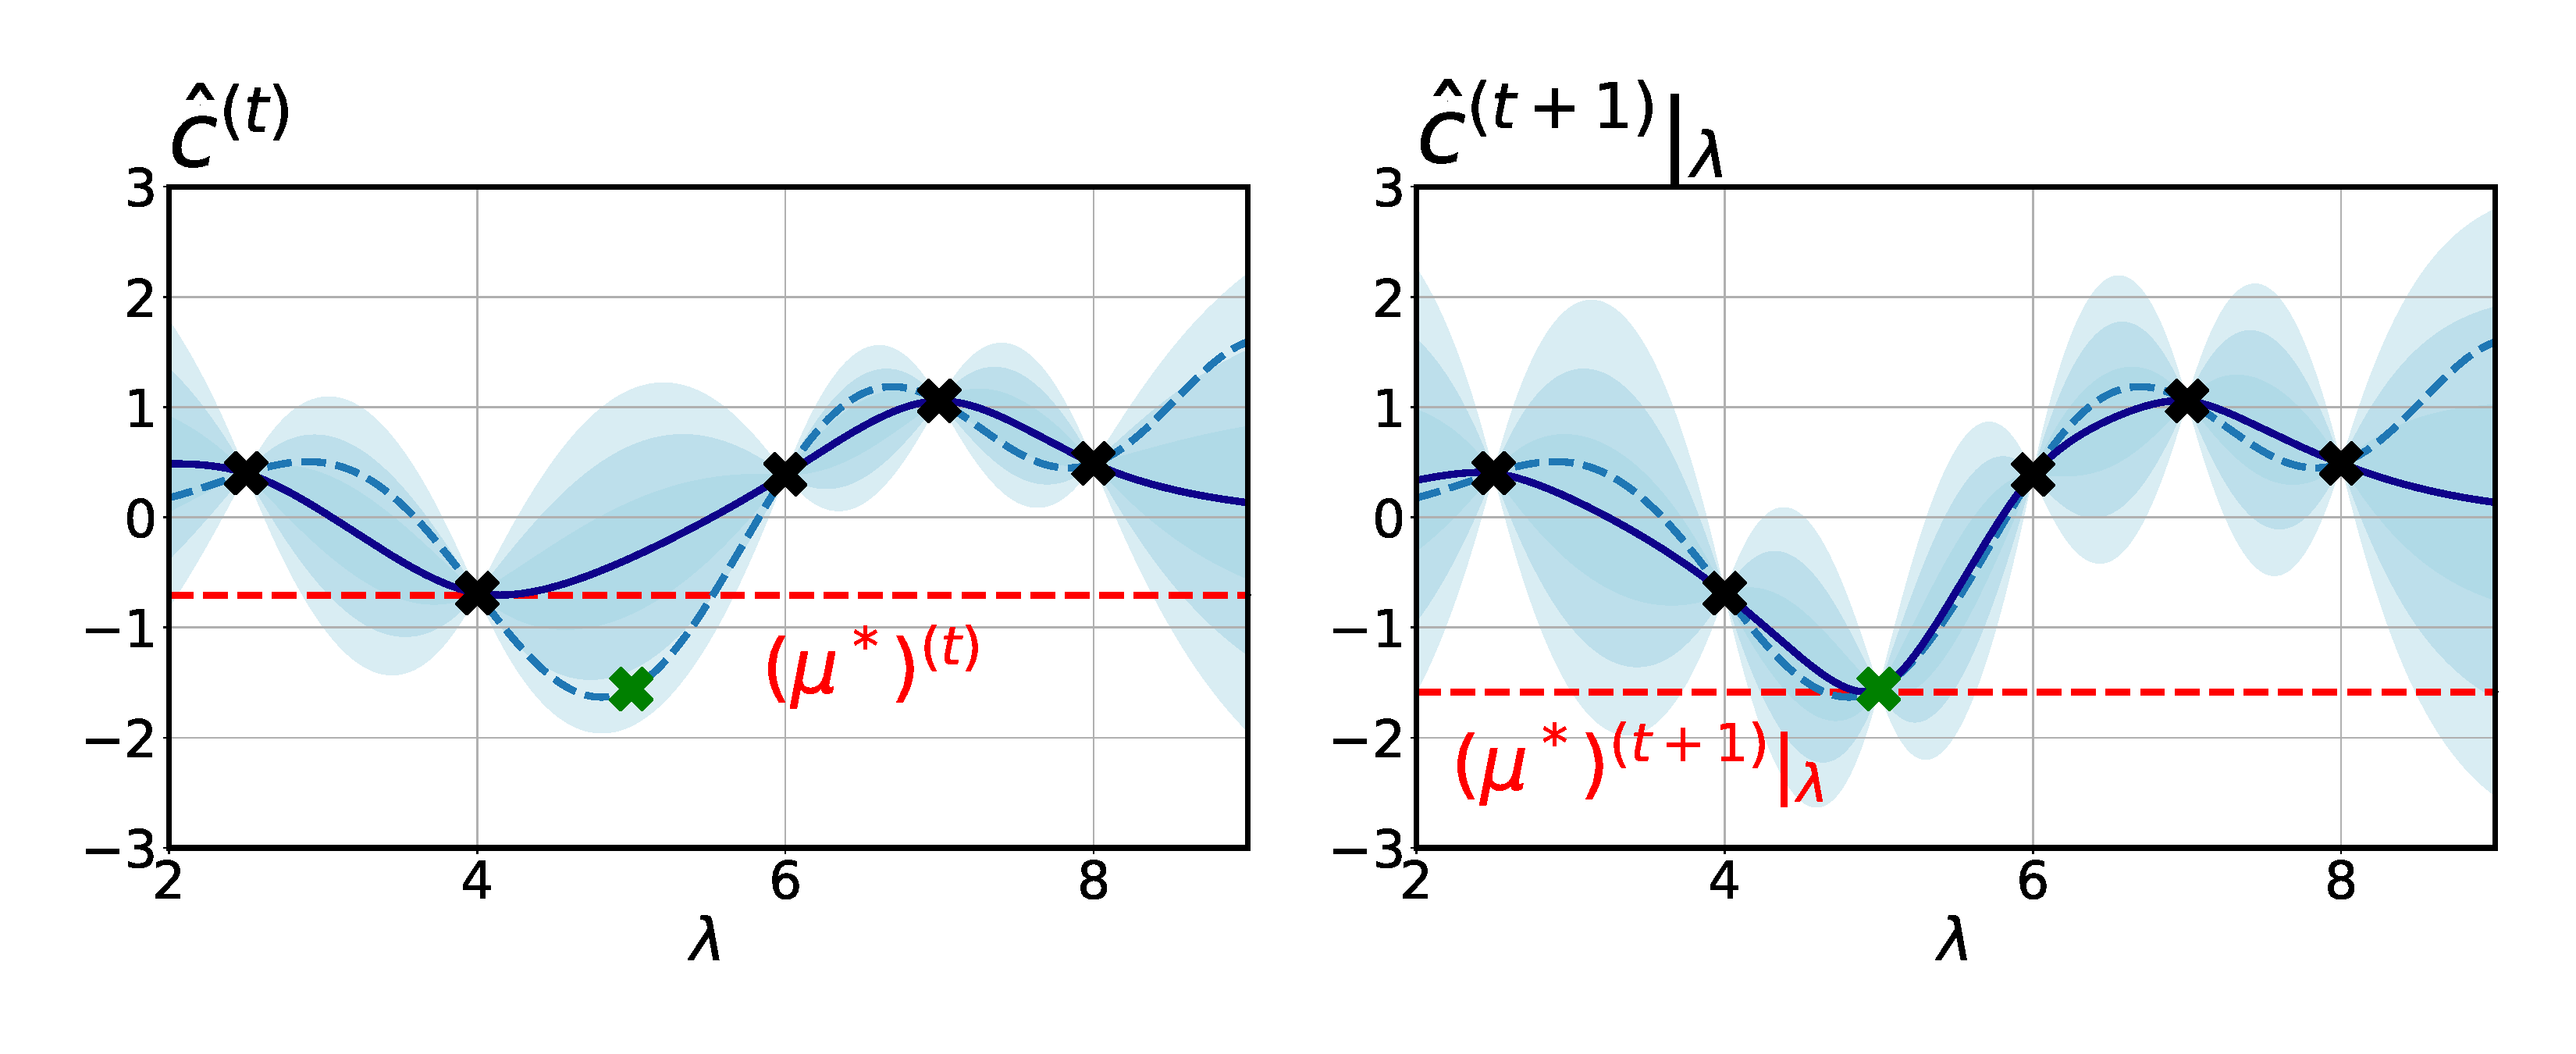
\includegraphics[width=\textwidth, height=0.7\textheight, keepaspectratio=true]{images/acq_func_images/kg/kg_5.pdf}}
\end{overlayarea}
\only<1>{Given the surrogate $\surro(\conf) = \normaldist( \mean(\conf), \variance(\conf))$
fit at iteration $\bocount$}

\only<2>{If we are risk-neutral, we'd return     $\arg\min_{\conf} \iter{\left(\mean(\conf)\right)}$ as incumbent, with \alert{value $\iter[\bocount]{\left(\mean^*\right)}$}}

\only<3>{If we perform a one-step look-ahead for configuration $\conf$, we would get     $\iter[\bocount+1]{\surro}{\!\given_{\!\conf}}$}

\only<4>{We would then be interested in the \alert{minimum of the updated mean function $\iter[\bocount+1]{\left(\mean^*\right)} \given_{\conf}$}}
%    The best risk-neutral choice would then the minimum of the new conditional mean function: $\iter[\bocount+1]{\left(\mean^*\right)} \given_{\conf}$.};

\only<5>{The \alert{Knowledge Gradient} is then the \alert{expectation of the improvement $\iter[\bocount+1]{\left(\mean^*\right)} - \iter[\bocount+1]{\left(\mean^*\right)} \!\given_{\!\conf}$}}
% \end{figure}

\end{frame}
%-----------------------------------------------------------------------
%\begin{frame}[c]{Knowledge Gradient (KG): Formal Definition (1/3)}
%\begin{itemize}\belowdisplayskip=1.5em
%    \item<+-> Given a GP $\iter{\gp}$ fit on $\iter[\bocount-1]{\dataset}$ on the $\bocount\,$th iteration, we have
%    \[
%        \iter{\left(\mean^*\right)} = \min_{\conf'\in\pcs}\,\iter{\mean}\left(\conf'\big|\iter[\bocount-1]{\dataset}\right)
%    \]
%    
%    \item<+-> If we choose a candidate $\bonextsample=\conf$ to evaluate $\cost(\cdot)$ at,
%    \[
%        \left.\iter{\dataset}\right|_{\conf} = \iter[\bocount-1]{\dataset}\cup\left\{\left\langle\bonextsample,\,\bonextobs\right\rangle\big|\bonextsample=\conf\right\}
%    \]
%    
%    \item <+-> Thus, if we hypothesize about the $\bocount+1\,$th iteration, we would get
%    \[
%        \begin{split}
%        \left.\iter[\bocount+1]{\left(\mean^*\right)} \right|_{\conf} 
%        &= \min_{\conf'\in\pcs} \iter[\bocount+1]{\mean} \left(\conf'\big| \iter{\dataset},\bonextsample=\conf \right)\\
%        %&= \min_{\conf'\in\pcs} \iter[\bocount+1]{\mean} \left(\conf'\big| \iter[\bocount-1]{\dataset},\conf,\obs \right)\\
%        \end{split}
%    \]
%\end{itemize}
%\comment{Source:https://arxiv.org/pdf/1807.02811.pdf}
%\end{frame}
%%-----------------------------------------------------------------------
%\begin{frame}[c]{Knowledge Gradient (KG): Formal Definition (2/3)}
%\begin{itemize}\belowdisplayskip=1.5em
%    \item<+->In a risk-neutral setting, $\iter{\left(\mean^*\right)}$ and $\left.\iter[\bocount+1]{\left(\mean^*\right)}\right|_{\conf}$ are the global optima for $\iter{\mean}$ and $\left.\iter[\bocount+1]{\mean}\right|_{\conf}$ respectively.
%    
%    \item<+-> Thus, the conditional improvement in the cost is 
%    \[
%        \left.\iter{I}\right|_{\conf}=\iter{\left(\mean^*\right)} - \left.\iter[\bocount+1]{\left(\mean^*\right)} \right|_{\bonextsample=\conf}
%    \]
%    
%    \item<+-> We cannot directly compute this improvement without performing an evaluation, but we can compute its expected value, which we call \emph{Knowledge Gradient}.
%    \lit{\href{https://arxiv.org/pdf/1807.02811.pdf}{Frazier 2018}}
%\end{itemize}
%\end{frame}
%-----------------------------------------------------------------------
\begin{frame}[c]{Knowledge Gradient (KG): Formal Definition}
\begin{itemize}\belowdisplayskip=1.5em
    
    \item The Knowledge Gradient is the \alert{expectation of the improvement $\iter[\bocount+1]{\left(\mean^*\right)} - \iter[\bocount+1]{\left(\mean^*\right)} \!\given_{\!\conf}$}:
    \[
    \begin{split}
        \iter{\acq}_{KG}(\conf) 
        &= \E\left[ \iter{\left(\mean^*\right)} - \left. \iter[\bocount+1]{\left(\mean^*\right)} \right|_{\bonextsample=\conf} \right]\\
        &=\min_{\conf'\in\pcs} \, \iter{\mean} \left(\conf' \big| \iter[\bocount-1]{\dataset} \right)
        - \E_{\tilde{\cost} \sim \iter[\bocount]{\surro(\lambda)}}
        %{p\left(\obs\big|\iter[\bocount-1]{\dataset},\conf\right)}
        \left[\min_{\conf'\in\pcs}\iter[\bocount+1]{\mean}\left(\conf'\given{\iter[\bocount-1]{\dataset} \cup \left\{\left\langle\conf, \tilde{\cost} \right\rangle \right\}}\right)\right]
    \end{split}
    \]
%\bigskip 
%\pause
%    \item Approximating the expectation is the expensive step; for an efficient approach, see \lit{\href{https://arxiv.org/pdf/1807.02811.pdf}{Frazier 2018}}
\pause
\bigskip
\[
    \boxed{\text{Choose}\;\;\bonextsample = \argmax_{\conf\in\pcs}(\iter{\acq}_{KG}(\conf))}
    \]
    \comment{\lit{\href{https://arxiv.org/pdf/1807.02811.pdf}{Frazier 2018}}}
\end{itemize}
\end{frame}



\begin{frame}[c]{Knowledge Gradient: Pseudocode for Monte Carlo Approximation}

\[\iter{\acq}_{KG}(\conf) = const - \alert{
\E_{\tilde{\cost} \sim \iter[\bocount]{\surro(\lambda)}}
        %{p\left(\obs\big|\iter[\bocount-1]{\dataset},\conf\right)}
        \left[\min_{\conf'\in\pcs}\iter[\bocount+1]{\mean}\left(\conf'\given{\iter[\bocount-1]{\dataset} \cup \left\{\left\langle\conf, \tilde{\cost} \right\rangle \right\}}\right)\right]
}\]

\begin{center}
\begin{minipage}{0.75\textwidth}
\comment{Fix algorithm numbering}
\begin{algorithm}[H]
    %\DontPrintSemicolon
    \LinesNumbered
%    \SetAlgoLined
    \setcounter{AlgoLine}{0}
    \SetKwInOut{Require}{Require}
    \SetKwInOut{Result}{Result}
    
    \Require{Surrogate $\surro$, candidate configuration $\conf$, dataset $\dataset$}
    \Result{Utility $\acq(\conf)$}
    
    \For{$s=1$ \KwTo $S$}{
        Sample $\tilde{c}_s \sim \surro(\conf)$\;
        
        Update $\surro$ with $\{\left\langle\conf, \tilde{c}_s\right\rangle\}$ to yield $\surro_s = \normaldist( \mean_s, \variance_s)$\;
        
        $e[s]\leftarrow  \min_{\conf'\in\pcs}{\mean_s}$
    }

    $\acq\leftarrow const - \frac{1}{S} \sum_{s=1}^S e[s]$\;

    \caption*{Sampling Based Knowledge Gradient Acquisition Function}
\end{algorithm}
\end{minipage}

\pause
\bigskip
This sampling view is useful for intuition;\\ but in practice, there are more efficient ways to optimize KG \lit{\href{https://arxiv.org/pdf/1807.02811.pdf}{Frazier 2018}}

\end{center}

\end{frame}

%-----------------------------------------------------------------------
\begin{frame}[c]{Entropy Search  Preliminaries}
\begin{itemize}
    \item Key idea: Evaluate $\conf$ which most \alert{reduces our uncertainty about the location of $\optconf$}
\bigskip    
\pause    
    \item We'll use the $p_{min}$ distribution to characterize the location of $\optconf$: \alert{\[p_{min}(\conf^*|\dataset) = p(\conf^* \in \argmin_{\conf' \in \pcs} (\surro(\conf') | \dataset))\]}
\medskip
\pause
    \item Our uncertainty is then captured by the \alert{entropy $H( p_{min}(\cdot |\dataset))$ of the $p_{min}$ distribution}
\pause
\bigskip    
    \item Minimizing $H( p_{min}(\cdot |\dataset))$ yields a peaked $p_{min}$ distribution, i.e., strong knowledge about the location of $\optconf$
    
%    Do this by minimizing the entropy of the distribution of the lowation of the minimum: $\mathcal{H}(p_{min})$
%    \item<+-> $p_{min}(\conf^*|\dataset) = p(\conf^* \in \argmin_{\conf' \in \pcs} (\surro(\conf') | \dataset))$
%    \item<+-> We define the acquisition function as 
%    \[
%    \begin{split}
%      \iter{\acq}_{ES}(\conf,\dataset) = \mathcal{H}\left(p_{min}(\conf^*)|\dataset \right) - \E_{\tilde{\cost} \sim \iter[\bocount]{\surro(\conf)}}\left[\mathcal{H} \left( p_{min}(\conf^*)|\dataset \cup \left\{ \left\langle \conf, \tilde{\cost} \right\rangle \right\} \right)\right]
%    \end{split}
%    \]
%    \item<+-> Entropy search contains a similar look-ahead as knoledge gradient
%    \item<+-> And as always, 
%    \[
%    \text{Choose}\,\boxed{\bonextsample = \argmax_{\conf\in\pcs}(\iter{\acq}_{ES}(\conf))}
%    \]
\end{itemize}

\end{frame}
%-----------------------------------------------------------------------
\begin{frame}[c]{Entropy Search: Visualization of the $p_{min}$ Distribution}

% \begin{figure}
  \centering
  \begin{tikzpicture}
%    \node<+> (img1) {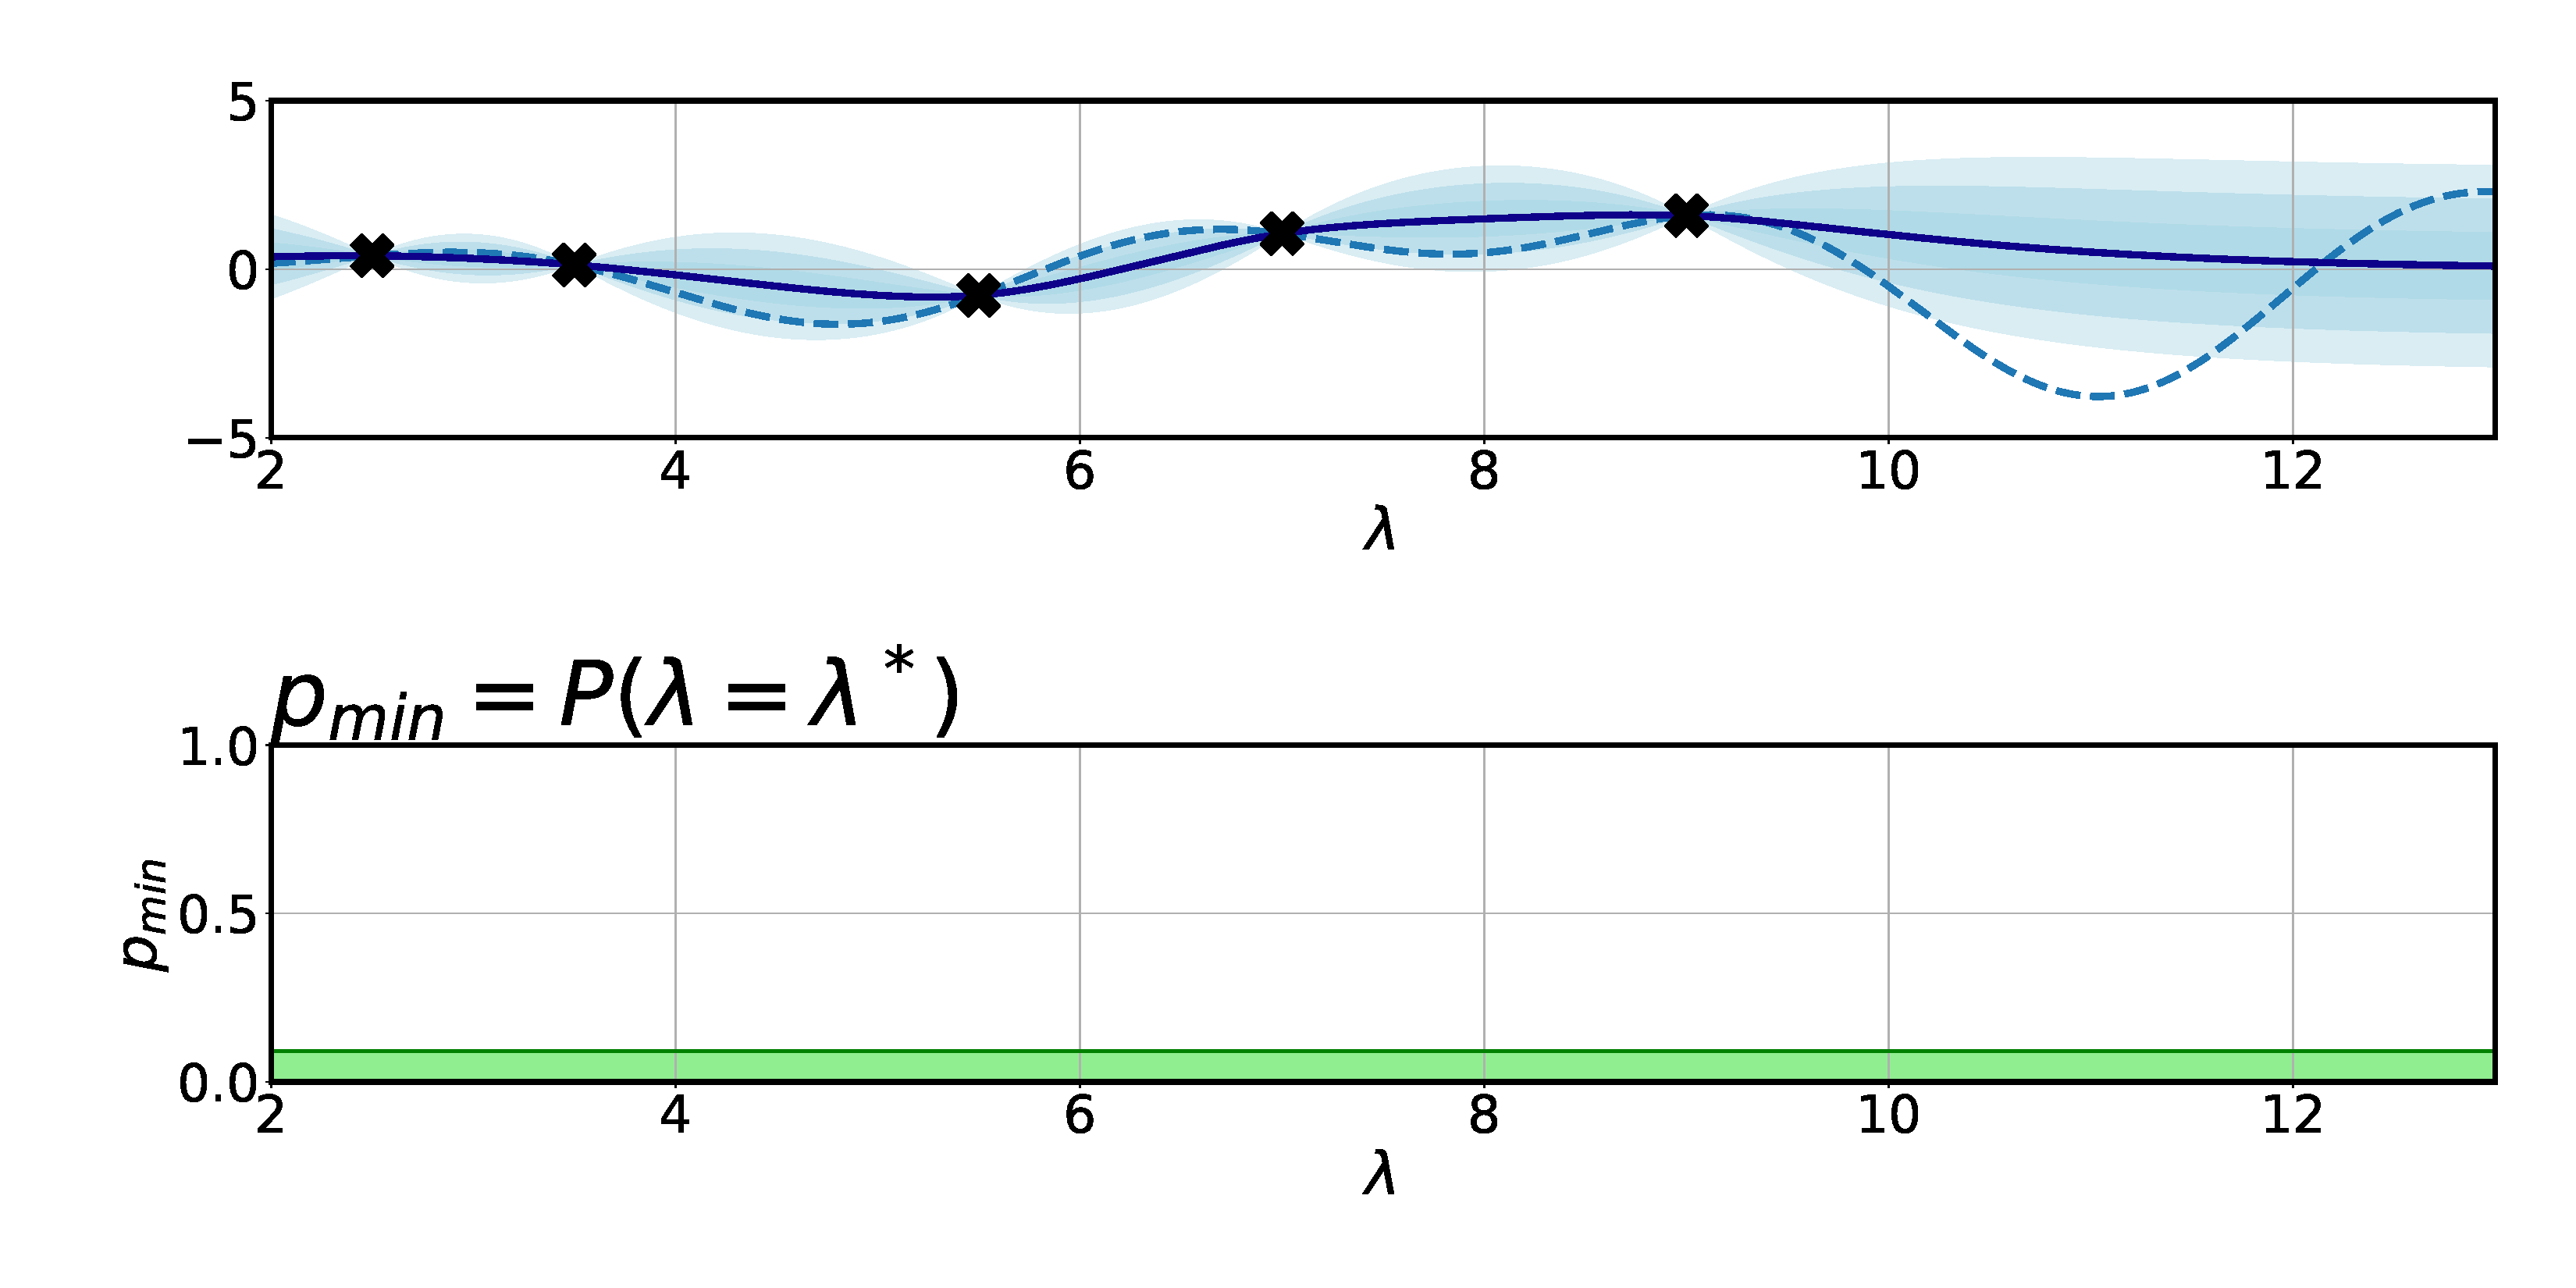
\includegraphics[width=\linewidth, height=0.7\textheight, keepaspectratio=true]{images/acq_func_images/es/es_1.pdf}};
%    \node<.> [below=-1.0\belowcaptionskip of img1, align=center]{
%    %We consider the global optimum's position to be a random variable $\conf^*$, \\ so each configuration $\conf$ can be assigned a probability $p_{min}=P(\conf=\conf^*)$.};
%    Initially, the $p_{min}$ distribution is uniform};
    
    \node<+> (img2) {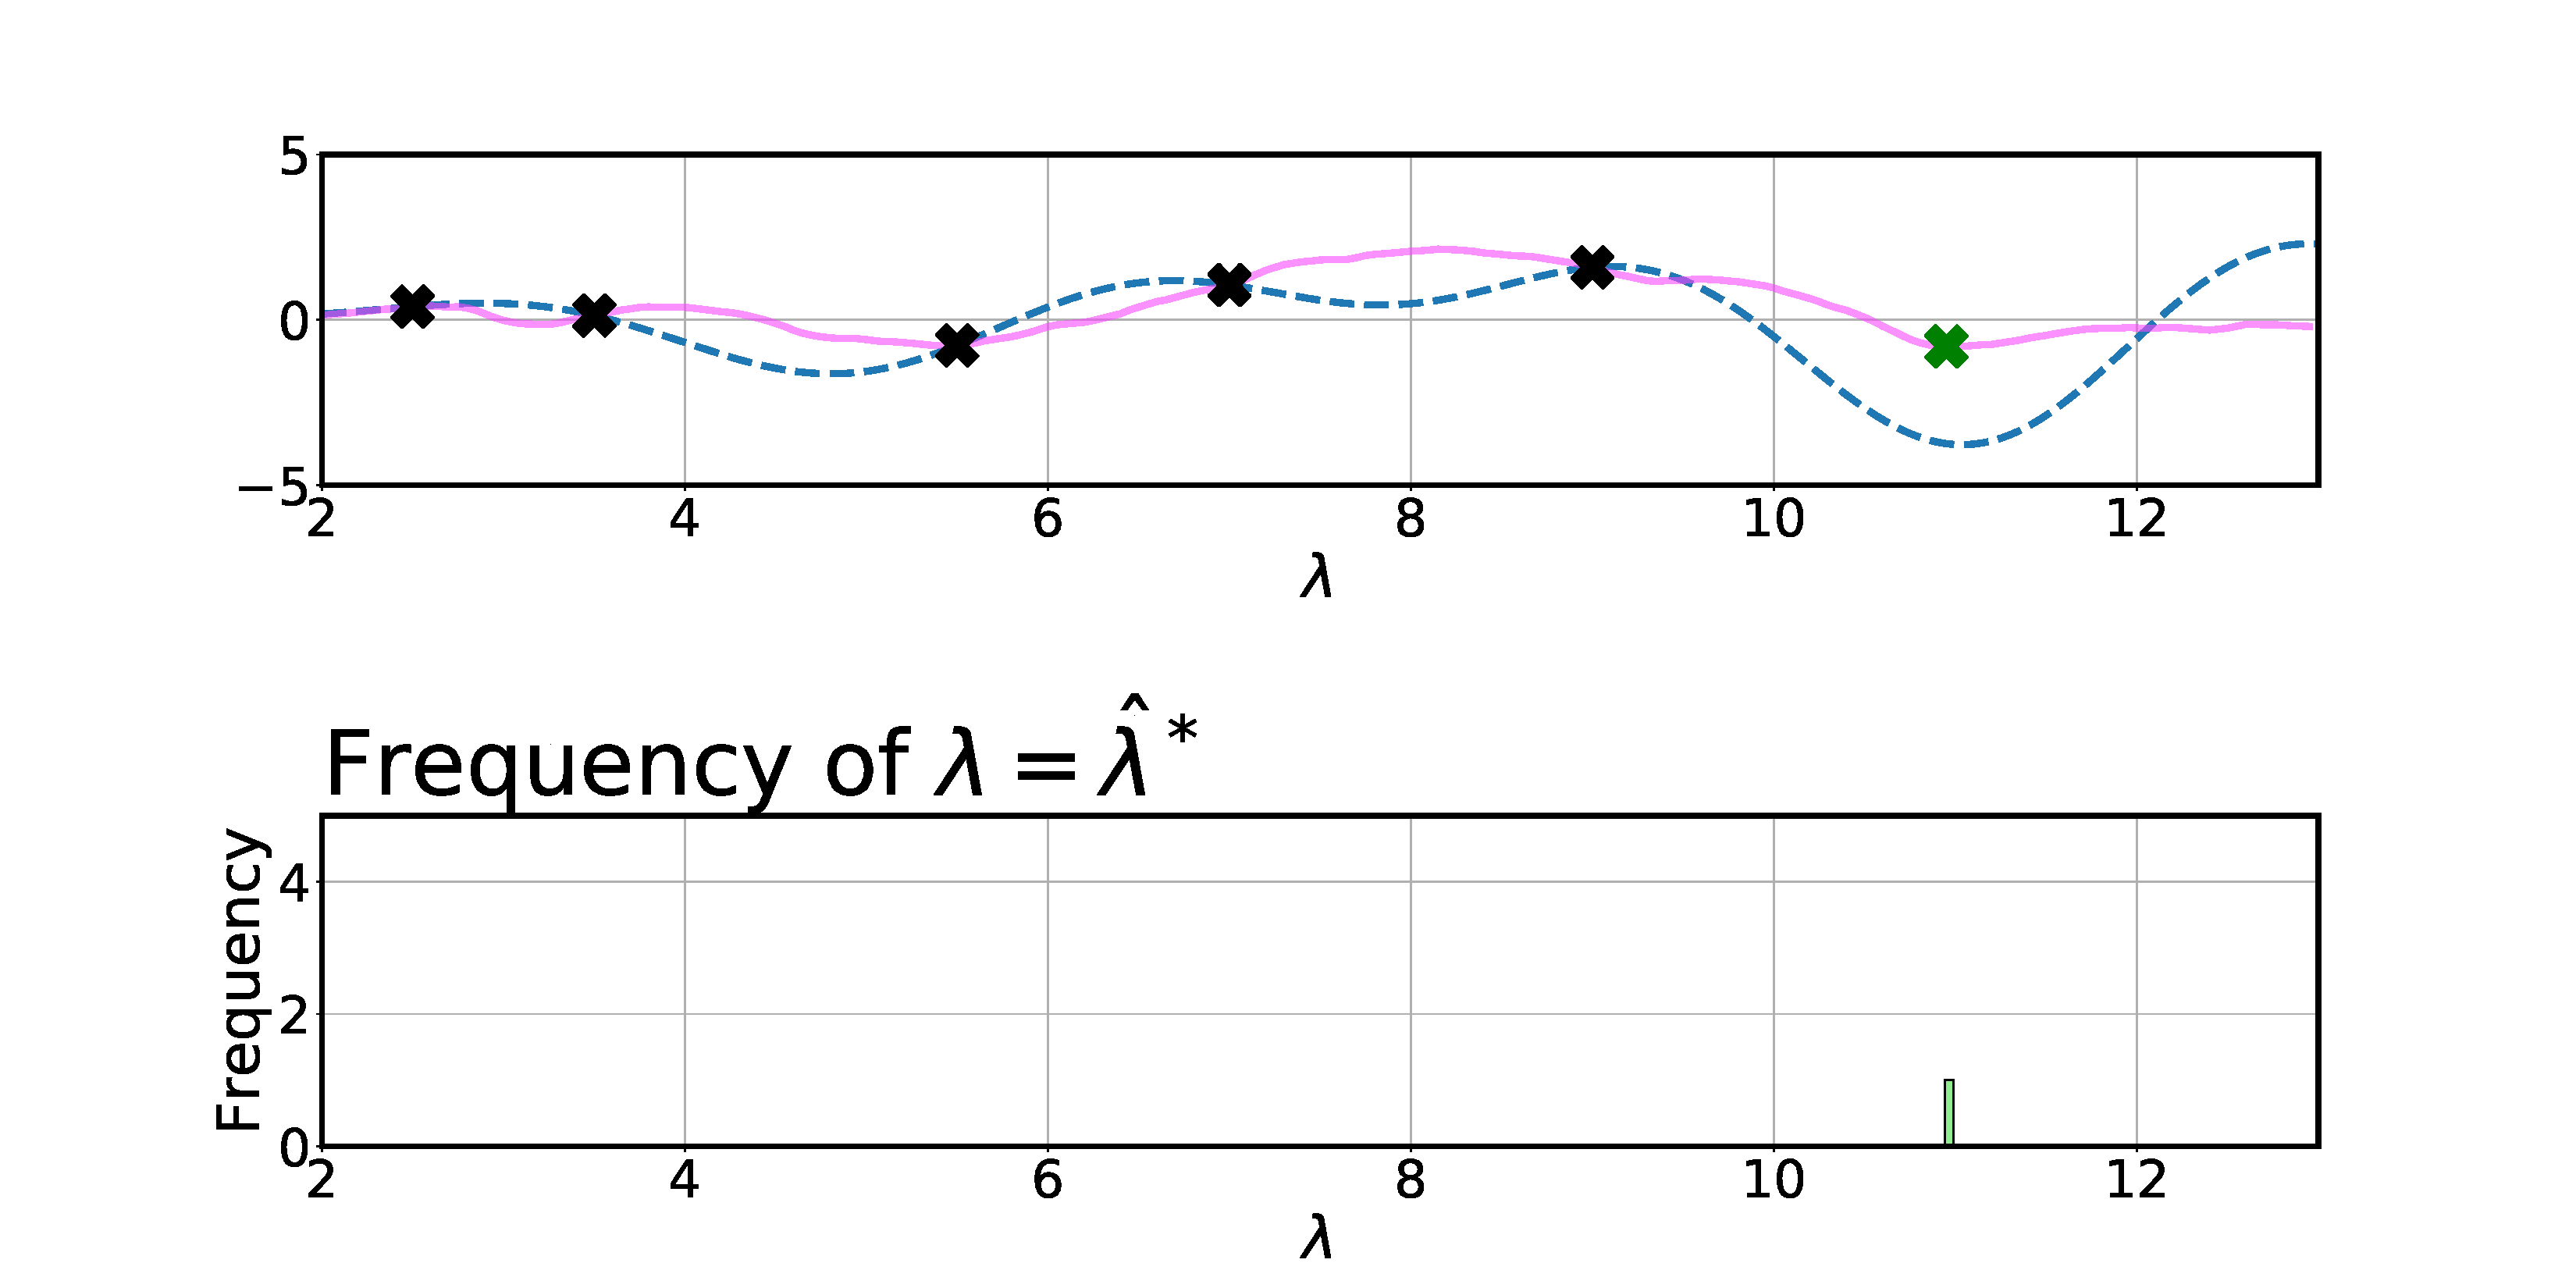
\includegraphics[width=\linewidth, height=0.7\textheight, keepaspectratio=true]{images/acq_func_images/es/es_2.pdf}};
    \node<.> [below=-1.0\belowcaptionskip of img2, align=center]{For each sample drawn from $\surro$, we can compute where $\conf^*$ lies};
    
    \node<+> (img3) {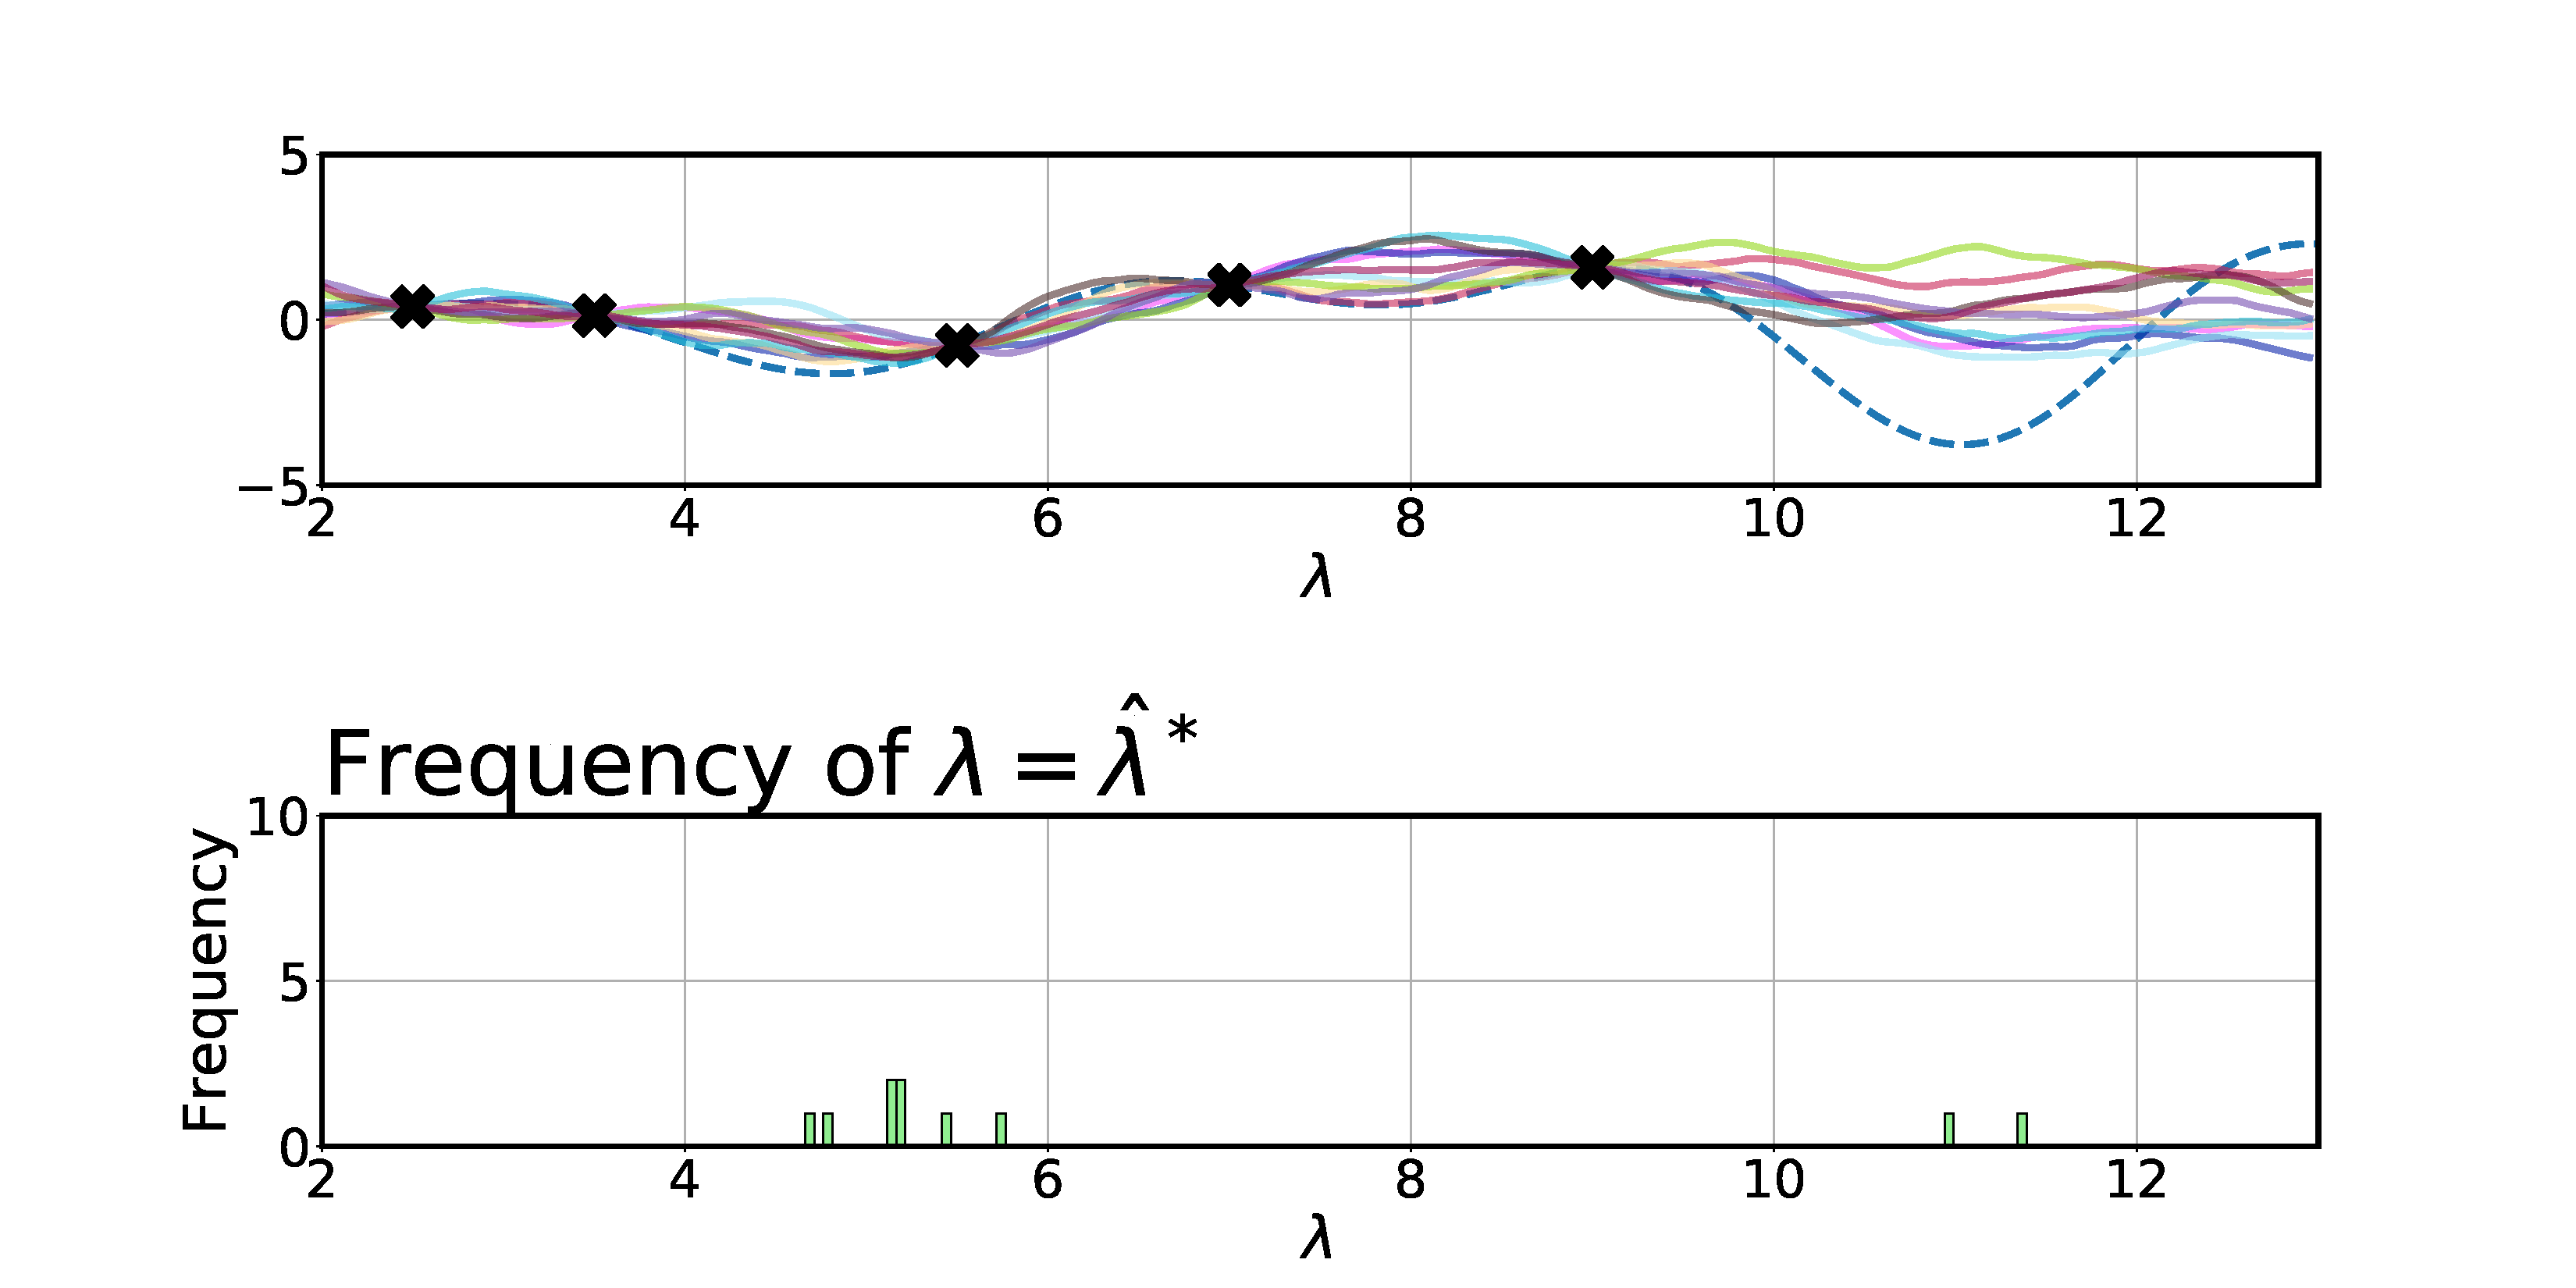
\includegraphics[width=\linewidth, height=0.7\textheight, keepaspectratio=true]{images/acq_func_images/es/es_3.pdf}};
    \node<.> [below=-1.0\belowcaptionskip of img3, align=center]{For each sample drawn from $\surro$, we can compute where $\conf^*$ lies};
    
    \node<+> (img4) {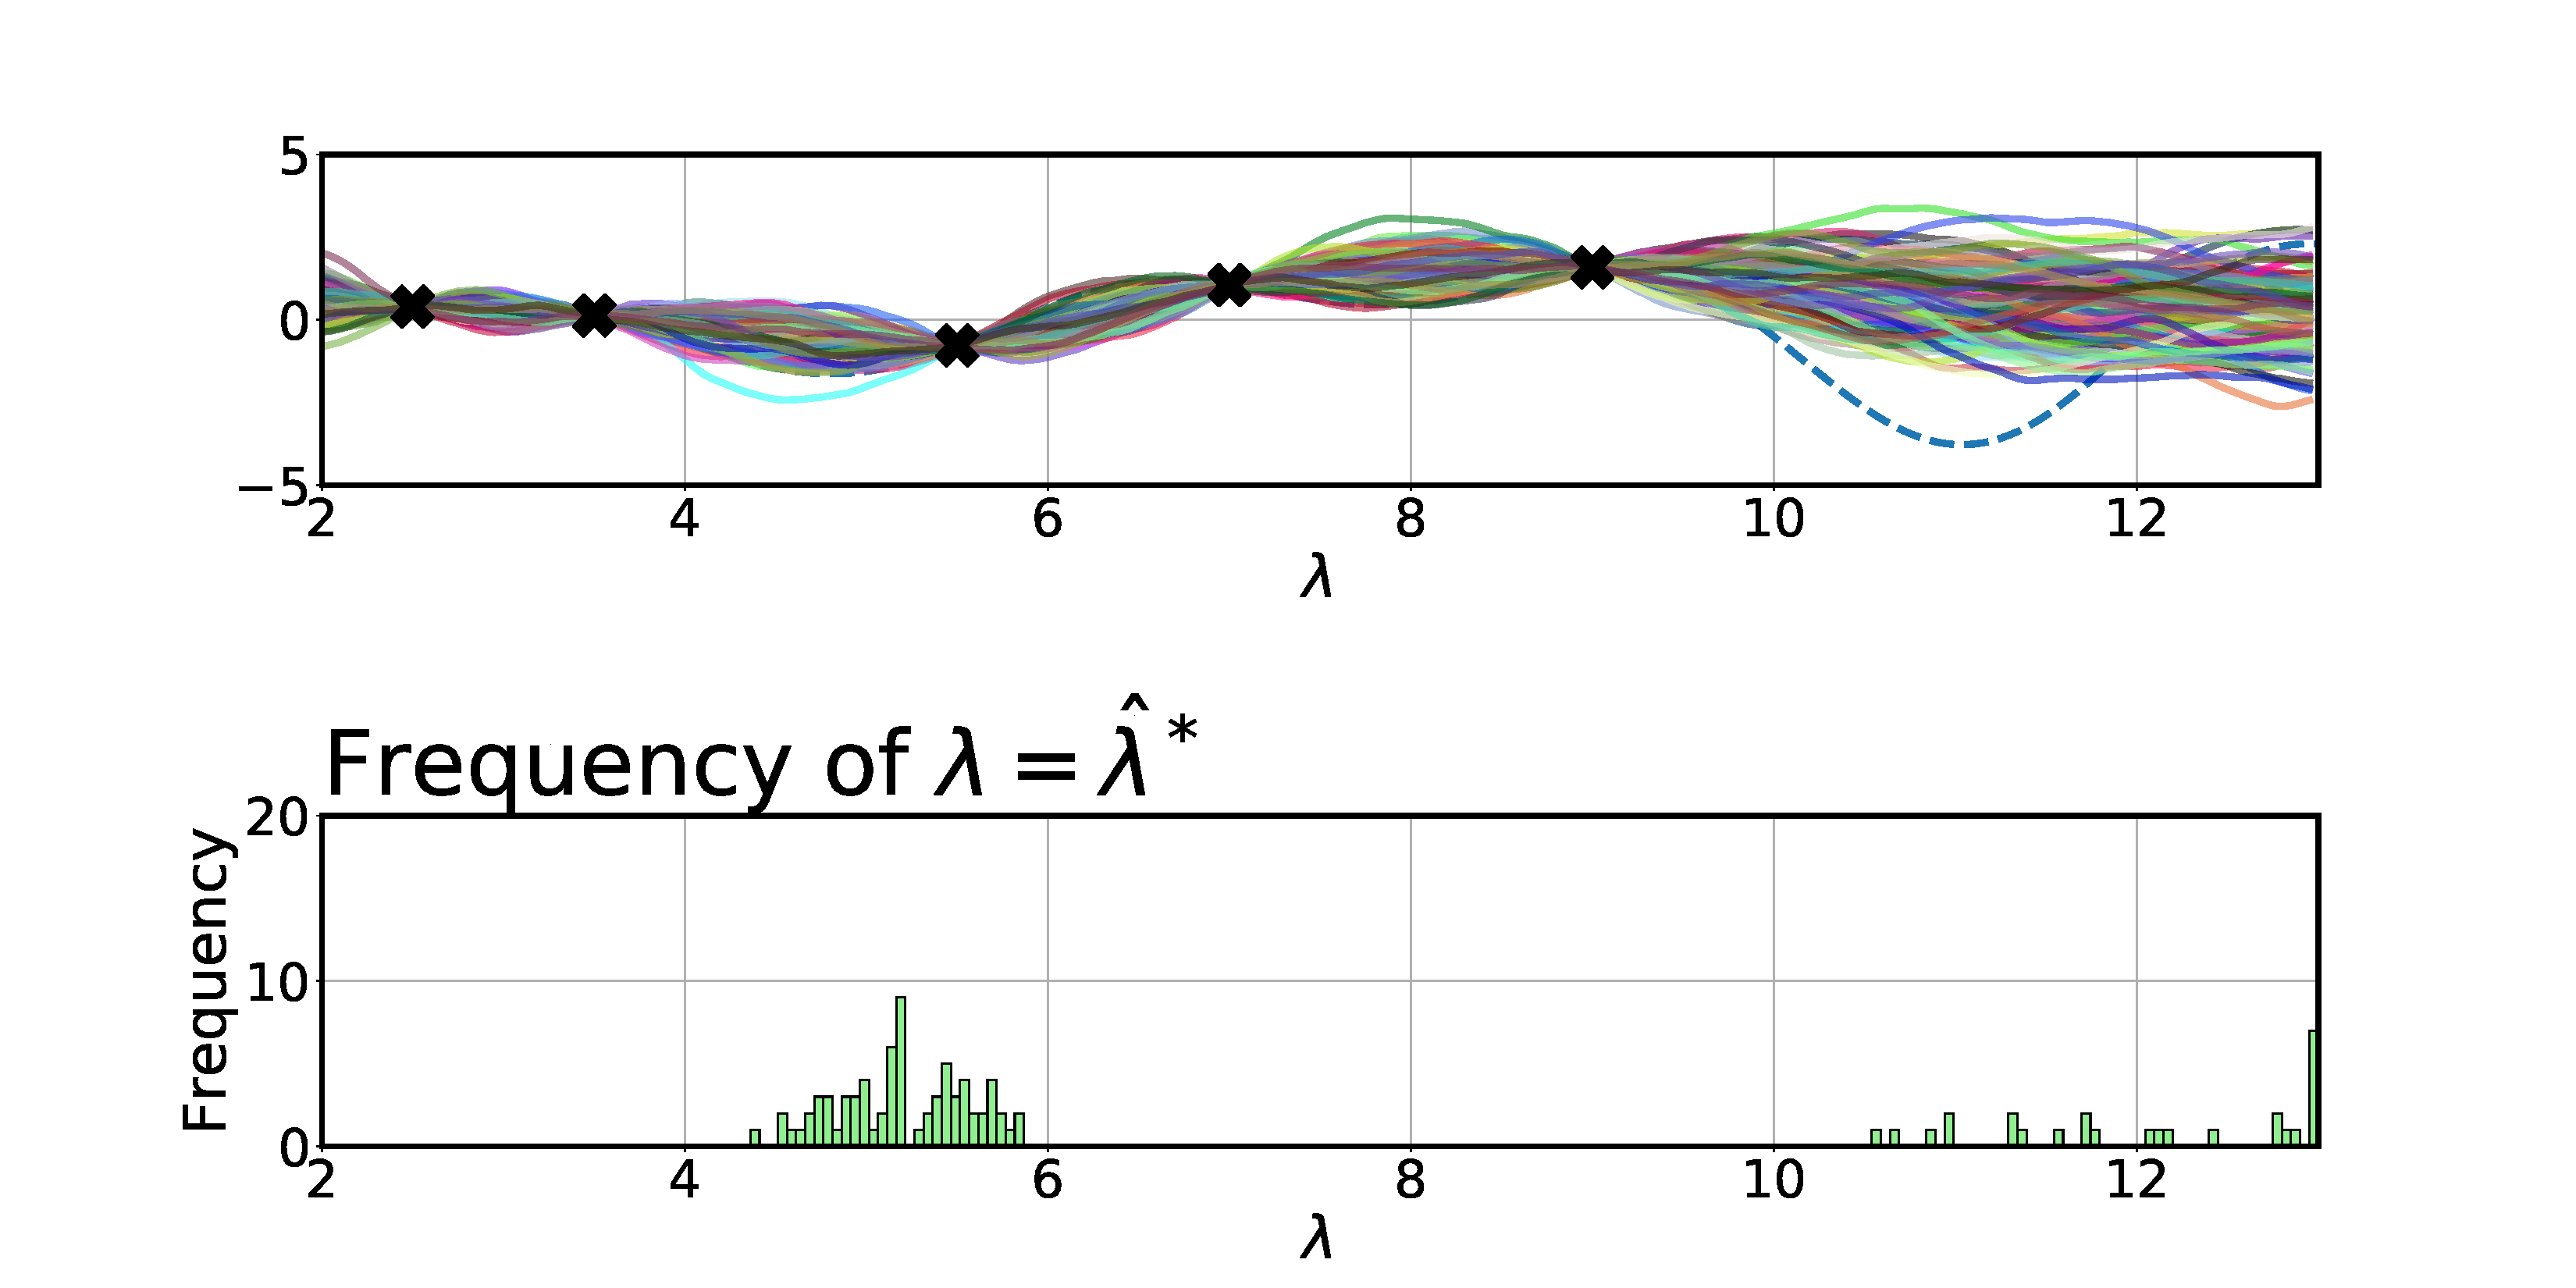
\includegraphics[width=\linewidth, height=0.7\textheight, keepaspectratio=true]{images/acq_func_images/es/es_4.pdf}};
    \node<.> [below=-1.0\belowcaptionskip of img4, align=center]{From many samples we can approximate the $p_{min}$ distribution};
    
    \node<+> (img5) {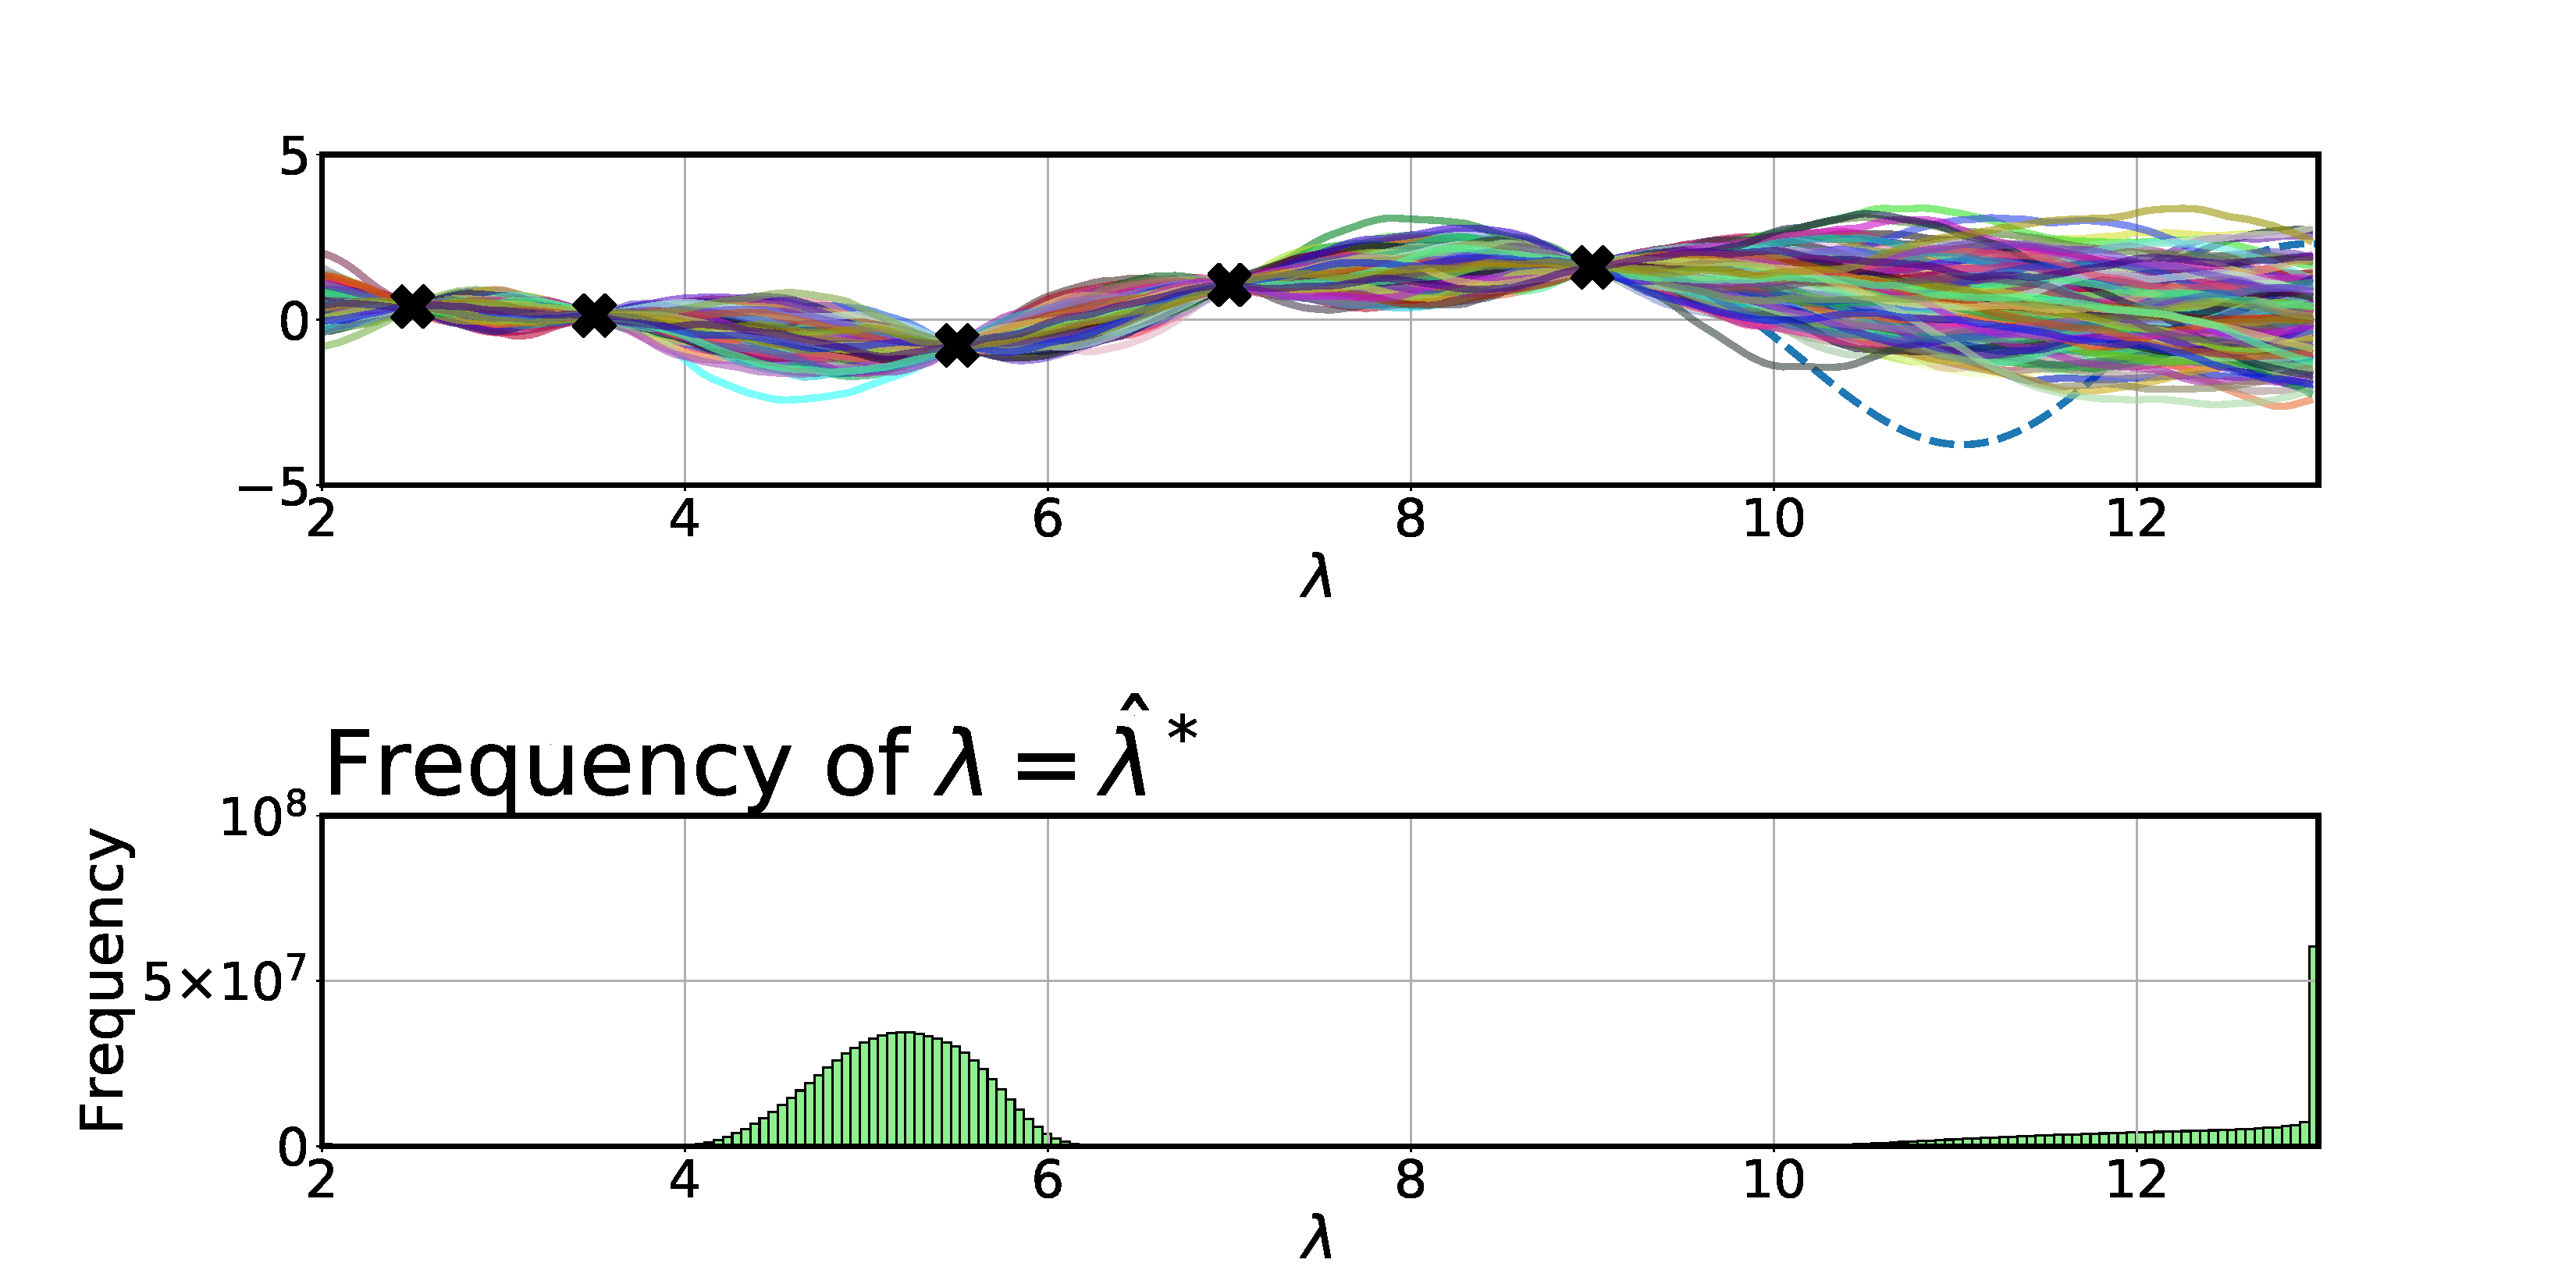
\includegraphics[width=\linewidth, height=0.7\textheight, keepaspectratio=true]{images/acq_func_images/es/es_5.pdf}};
    \node<.> [below=-1.0\belowcaptionskip of img5, align=center]{From many samples we can approximate the $p_{min}$ distribution};
%    \comment{Since the aim was to illustrate a concept, the underlying code for these plots used simplified max-value entropy search, and the final PDF was generated using Kernel Density Estimation, thus leading to an artifact at the right edge where a very high bin value was "lost".
%    }
    
%    \node<+> (img6) {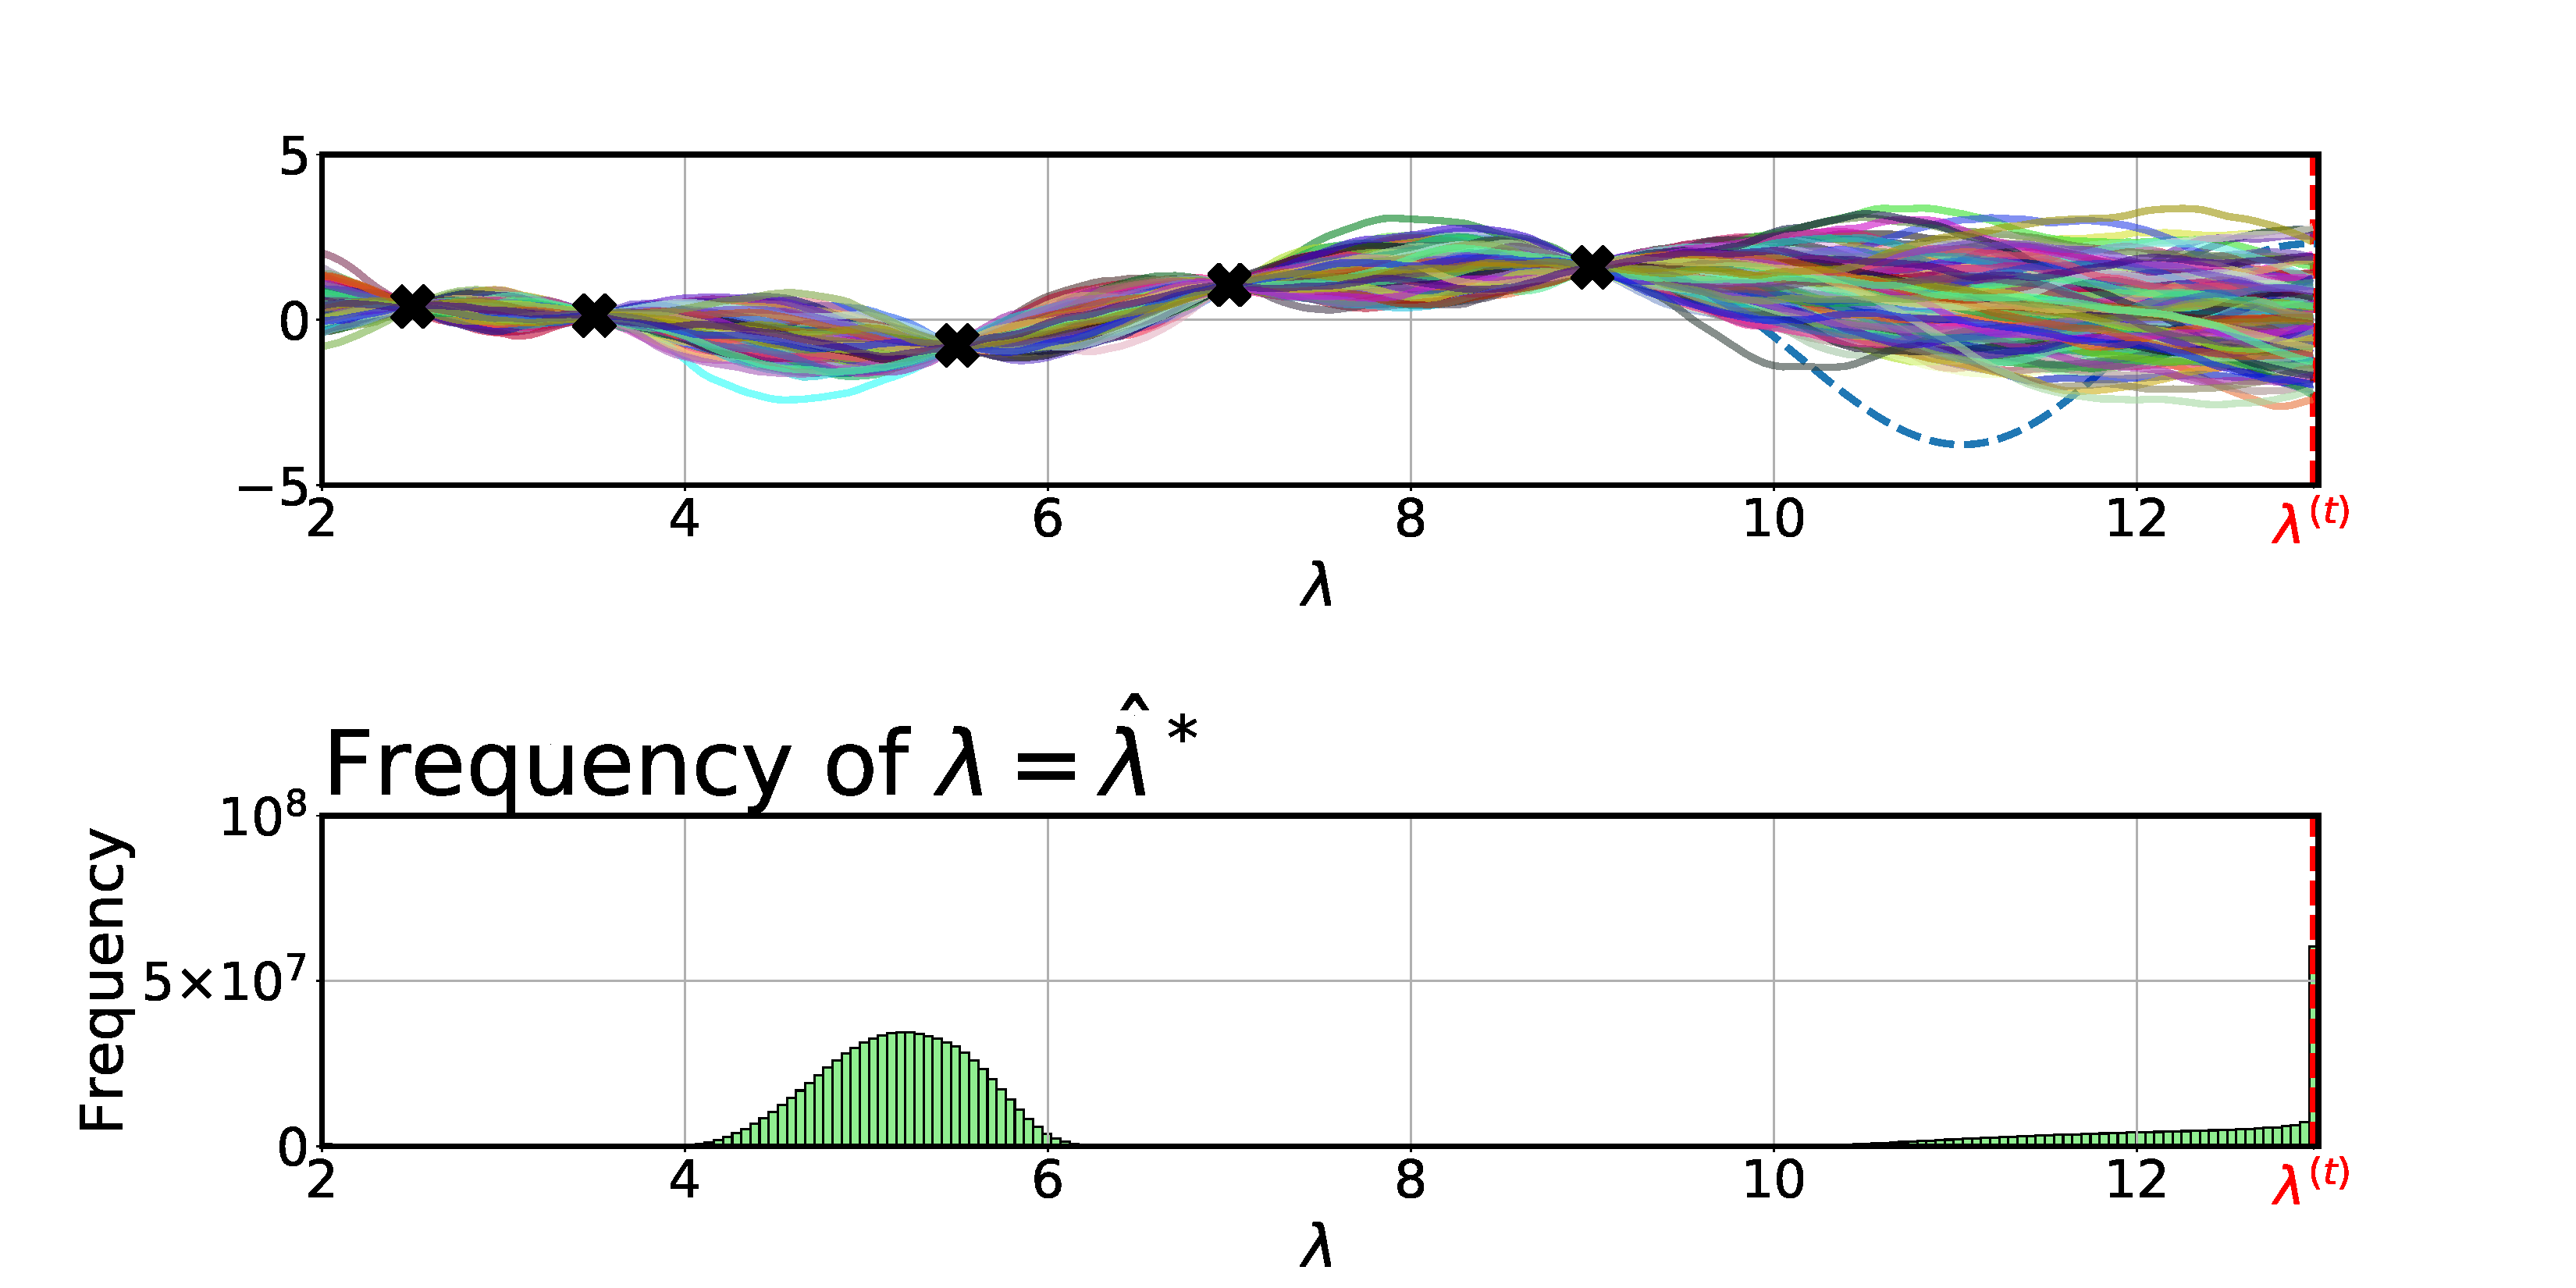
\includegraphics[width=\linewidth, height=0.7\textheight, keepaspectratio=true]{images/acq_func_images/es/es_6.pdf}};
%    \node<.> [below=-1.0\belowcaptionskip of img6, align=center]{
    %FH: this is still WRONG, I commented out the slide! %The configuration that is most likely to be $\conf^*$ provides the greatest information gain,\\ or in other words, would reduce the entropy of the search space the most when evaluated.};
    
  \end{tikzpicture}
% \end{figure}

% \notefh{The figures should not jump around the slide in a PDF animation.}

\end{frame}

%-----------------------------------------------------------------------
\begin{frame}[c]{Entropy Search: Formal Definition}
\begin{itemize}

    \item The $p_{min}$ distribution characterizes the location of $\optconf$: \alert{\[p_{min}(\conf^*|\dataset) = p(\conf^* \in \argmin_{\conf' \in \pcs} (\surro(\conf') | \dataset))\]}
\smallskip
\pause
    \item Our uncertainty about the location of $\optconf$ is captured by the \alert{entropy $H( p_{min}(\cdot |\dataset))$ of the $p_{min}$ distribution}
\bigskip    
\pause
\item \alert{Entropy search aims to minimize $H(p_{min})$}, to yield a peaked $p_{min}$ distribution:
    %, i.e., strong knowledge about the location of $\optconf$:
    
    \alert{\[u_{ES}(\conf) = H( p_{min}(\cdot |\dataset)) - \E_{\tilde{\cost} \sim \iter[\bocount]{\surro(\lambda)}} H( p_{min}(\cdot |\dataset \cup \left\{\left\langle\conf, \tilde{\cost} \right\rangle \right\})) \]}
    
%    Do this by minimizing the entropy of the distribution of the lowation of the minimum: $\mathcal{H}(p_{min})$
%    \item<+-> $p_{min}(\conf^*|\dataset) = p(\conf^* \in \argmin_{\conf' \in \pcs} (\surro(\conf') | \dataset))$
%    \item<+-> We define the acquisition function as 
%    \[
%    \begin{split}
%      \iter{\acq}_{ES}(\conf,\dataset) = \mathcal{H}\left(p_{min}(\conf^*)|\dataset \right) - \E_{\tilde{\cost} \sim \iter[\bocount]{\surro(\conf)}}\left[\mathcal{H} \left( p_{min}(\conf^*)|\dataset \cup \left\{ \left\langle \conf, \tilde{\cost} \right\rangle \right\} \right)\right]
%    \end{split}
%    \]
%    \item<+-> Entropy search contains a similar look-ahead as knoledge gradient
%    \item<+-> And as always, 
    \[
    \boxed{\text{Choose}\;\;\bonextsample = \argmax_{\conf\in\pcs}(\iter{\acq}_{ES}(\conf))}
    \]
\end{itemize}

\end{frame}
%-----------------------------------------------------------------------

% %----------------------------------------------------------------------
% \begin{frame}[c]{Computationally Expensive Acquisition Functions - ES}
% \framesubtitle{Entropy Search - Pseudocode for Sampling Version}

% \begin{center}
% \begin{minipage}{0.75\textwidth}
% \comment{Fix algorithm numbering}
% \begin{algorithm}[H]
%     %\DontPrintSemicolon
%     \LinesNumbered
%     \SetAlgoLined
%     \setcounter{AlgoLine}{0}
%     \SetKwInOut{Require}{Require}
%     \SetKwInOut{Result}{Result}
    
%     \Require{GP $\iter{\gp}$, budget $S$}
%     \Result{$\bonextsample$}
    
%     $E\leftarrow{\langle E_{\conf} = 0 \rangle}_{\conf\in\pcs}$\;
    
%     \For{$s=1$ \KwTo $S$}{
    
%         Sample $g_s\sim\iter{\gp}$\;
        
%         $\conf_s\leftarrow\argmin(g_s)$\;
        
%         $E[\conf_s]\leftarrow E[\conf_s] + 1$\;\tcp{Update Histogram count}}

%     $\acq\leftarrow\mathcal{\hat{P}}(E)$\tcp*{Generate PDF from histogram $E$}\;
%     $\bonextsample\leftarrow\argmax_{\conf\in\pcs}u(\conf)$\;

%     \caption{Sampling Based Entropy Search}
% \end{algorithm}
% \end{minipage}
% \end{center}

% \end{frame}
%-----------------------------------------------------------------------
\begin{frame}[c]{Entropy Search: Pseudocode for Monte Carlo Approximation}

\vspace*{-0.2cm}
\[u_{ES}(\conf) = const - \alert{\E_{\tilde{\cost} \sim \iter[\bocount]{\surro(\lambda)}} H( p_{min}(\cdot |\dataset \cup \left\{\left\langle\conf, \tilde{\cost} \right\rangle \right\}))} \]
\vspace*{-0.5cm}

\begin{center}
\begin{minipage}{0.9\textwidth}
\comment{Fix algorithm numbering}
\begin{algorithm}[H]
\footnotesize{}
    %\DontPrintSemicolon
    \LinesNumbered
%    \SetAlgoLined
    \setcounter{AlgoLine}{0}
    \SetKwInOut{Require}{Require}
    \SetKwInOut{Result}{Result}
    
    \Require{Surrogate $\surro$, candidate configuration $\conf$, finite set of representer points $\pcs_{r}$, dataset $\dataset$}
    \Result{Utility $\acq(\conf)$}
    
    
    \For{$s=1$ \KwTo $S$}{
    %Sample $\tilde{c}_s \sim \normaldist(\conf | \mu_{\iter{\gp}}, \sigma_{\iter{\gp}})$\;
        Sample $\tilde{c}_s \sim \surro(\conf)$; \;
        $\surro_s \leftarrow $ Update $\surro$ with 
        $\{\left\langle\conf, \tilde{c}_s\right\rangle\}$\;

        Initialize $F[\conf]=0$ $\;\; \forall \conf'\in\pcs_{r}$

        \For{$n=1$ \KwTo $N$}
        {
           Sample $g_n\sim\surro_s$\;
           
           $\conf_s\leftarrow\argmin_{\conf' \in \pcs_{r}} g_n$\;
           
            $F[\conf_s]\leftarrow 
            F[\conf_s] + 1$\;   
        }
        $p_{min,s}(\conf') \leftarrow F_{\conf'} / N \;\;\; \forall{\conf' \in \pcs_{r}} $ \;
        
        $H_s \leftarrow H(p_{min,s}) \text{, computed as } - \sum_{\conf' \in \pcs_{r}} p_{min,s}(\conf') \log p_{min,s}(\conf')$\;
    }
    $\acq\leftarrow const - \frac{1}{S} \sum_{s=1}^{S} H_s$
    
    \caption*{Sampling Based Entropy Search Acquisition Function}
\end{algorithm}
\end{minipage}
\end{center}

\end{frame}
%----------------------------------------------------------------------
\begin{frame}[c]{Entropy Search: Variations}
\begin{itemize}
    %\item<+-> Note how repeated Thompson Sampling inherently approximates sampling based entropy-search!
    \item The sample-based approximation is slow; for a faster approximation with expectation propagation see the original ES paper  \lit{\href{http://jmlr.csail.mit.edu/papers/volume13/hennig12a/hennig12a.pdf}{Hennig et al. 2012}}
\medskip
    \item \alert{Predictive Entropy Search}  \lit{\href{http://papers.nips.cc/paper/5324-predictive-entropy-search-for-efficient-global-optimization-of-black-box-functions.pdf}{Hernández-Lobato et al. 2014}} is a frequently-used equivalent formulation that gives rise to more convenient approximations 
\medskip
    \item \alert{Max-Value Entropy Search} 
    \lit{\href{https://arxiv.org/abs/1703.01968}{Wang and Jegelka 2017}} is a recent variant that 
    is cheaper to compute and has similar behavior 
\medskip
    \item Further reading and summary for ES: \lit{\href{https://arxiv.org/pdf/1602.01064.pdf}{Metzen 2016}}
\end{itemize}
\end{frame}
%-----------------------------------------------------------------------
\begin{frame}[c]{Questions to Answer for Yourself / Discuss with Friends}
\begin{itemize}
    %KG
    \item \alert{Repetition.} Describe the similarities and differences between KG and EI.
\medskip
    %ES
    \item \alert{Discussion.} When is there an incentive for entropy search to sample at $\max(p_{min})$? 
%    \item \emph{Discussion.} How would you optimize the acquisition function in practice?
\end{itemize}
\end{frame}